%% abtex2-modelo-trabalho-academico.tex, v-1.9.2 laurocesar
%% Copyright 2012-2014 by abnTeX2 group at http://abntex2.googlecode.com/ 
%%
%% This work may be distributed and/or modified under the
%% conditions of the LaTeX Project Public License, either version 1.3
%% of this license or (at your option) any later version.
%% The latest version of this license is in
%%   http://www.latex-project.org/lppl.txt
%% and version 1.3 or later is part of all distributions of LaTeX
%% version 2005/12/01 or later.
%%
%% This work has the LPPL maintenance status `maintained'.
%% 
%% The Current Maintainer of this work is the abnTeX2 team, led
%% by Lauro César Araujo. Further information are available on 
%% http://abntex2.googlecode.com/
%%
%% This work consists of the files abntex2-modelo-trabalho-academico.tex,
%% abntex2-modelo-include-comandos and abntex2-modelo-references.bib
%%

% ------------------------------------------------------------------------
% ------------------------------------------------------------------------
% abnTeX2: Modelo de Trabalho Academico (tese de doutorado, dissertacao de
% mestrado e trabalhos monograficos em geral) em conformidade com 
% ABNT NBR 14724:2011: Informacao e documentacao - Trabalhos academicos -
% Apresentacao
% ------------------------------------------------------------------------
% ------------------------------------------------------------------------

\documentclass[
	% -- opções da classe memoir --
	12pt,				% tamanho da fonte
	openright,			% capítulos começam em pág ímpar (insere página vazia caso preciso)
	oneside,			% para impressão em verso e anverso. Oposto a oneside
	a4paper,			% tamanho do papel. 
	% -- opções da classe abntex2 --
	%chapter=TITLE,		% títulos de capítulos convertidos em letras maiúsculas
	%section=TITLE,		% títulos de seções convertidos em letras maiúsculas
	%subsection=TITLE,	% títulos de subseções convertidos em letras maiúsculas
	%subsubsection=TITLE,% títulos de subsubseções convertidos em letras maiúsculas
	% -- opções do pacote babel --
	english,			% idioma adicional para hifenização
	brazil				% o último idioma é o principal do documento
	]{dissertacao-ufrgs-abntex2}

% ---
% Pacotes básicos 
% ---
\usepackage{lmodern}			% Usa a fonte Latin Modern			
\usepackage[T1]{fontenc}		% Selecao de codigos de fonte.
\usepackage[utf8]{inputenc}		% Codificacao do documento (conversão automática dos acentos)
\usepackage{lastpage}			% Usado pela Ficha catalográfica
\usepackage{indentfirst}		% Indenta o primeiro parágrafo de cada seção.
\usepackage{color}				% Controle das cores
\usepackage{graphicx}			% Inclusão de gráficos
\usepackage{microtype} 			% para melhorias de justificação
\usepackage{mathtools, amsmath, amssymb, amsthm, latexsym}
\usepackage{lscape}
%\usepackage{geometry}
%\usepackage{Sweave}
% ---
% comentários
\usepackage[colorinlistoftodos]{todonotes}		
% ---

% ---
% Pacotes de citações
% ---
\usepackage[brazilian,hyperpageref]{backref}	 % Paginas com as citações na bibl
\usepackage[alf]{abntex2cite}	% Citações padrão ABNT

% --- 
% CONFIGURAÇÕES DE PACOTES
% --- 

% ---
% Configurações do pacote backref
% Usado sem a opção hyperpageref de backref
\renewcommand{\backrefpagesname}{Citado na(s) página(s):~}
% Texto padrão antes do número das páginas
\renewcommand{\backref}{}
% Define os textos da citação
\renewcommand*{\backrefalt}[4]{
	\ifcase #1 %
		Nenhuma citação no texto.%
	\or
		Citado na página #2.%
	\else
		Citado #1 vezes nas páginas #2.%
	\fi}%
% ---

% ---
% Informações de dados para CAPA e FOLHA DE ROSTO
% ---
\titulo{ESTIMAÇÃO DA ESTRUTURA A TERMO DA TAXA DE JUROS COM ABORDAGEM DE DADOS FUNCIONAIS}
\autor{Marcelo Castiel Ruas}
\local{Porto Alegre}
\data{2014}
\orientador{Prof. Dr. Hudson da Silva Torrent}
\coorientador{Prof. Dr. João Frois Caldeira}
\instituicao{%
  UNIVERSIDADE FEDERAL DO RIO GRANDE DO SUL
  \\
  FACULDADE DE CIÊNCIAS ECONÔMICAS
  \\
  PROGRAMA DE PÓS-GRADUAÇÃO EM ECONOMIA
  }
  %  Universidade Federal do Rio Grande do Sul
  %  Faculdade de Ciências Econômicas
  %  Programa de Pós-Graduação em Economia
\tipotrabalho{Dissertação (Mestrado)}
% O preambulo deve conter o tipo do trabalho, o objetivo, 
% o nome da instituição e a área de concentração 
\preambulo{Dissertação submetida ao Programa de Pós-Graduação em Economia da Faculdade  
 de Ciências Econômicas da UFRGS, 
como quesito parcial para obtenção do  
 título de Mestre em Economia, com ênfase em Economia Aplicada.}
% ---




% ---
% Configurações de aparência do PDF final

% alterando o aspecto da cor azul
\definecolor{blue}{RGB}{41,5,195}

% informações do PDF
\makeatletter
\hypersetup{
     	%pagebackref=true,
		pdftitle={\@title}, 
		pdfauthor={\@author},
    	pdfsubject={\imprimirpreambulo},
	    pdfcreator={LaTeX with abnTeX2},
		pdfkeywords={abnt}{latex}{abntex}{abntex2}{trabalho acadêmico}, 
		colorlinks=true,       		% false: boxed links; true: colored links
    	linkcolor=blue,          	% color of internal links
    	citecolor=blue,        		% color of links to bibliography
    	filecolor=magenta,      		% color of file links
		urlcolor=blue,
		bookmarksdepth=4
}
\makeatother
% --- 

% --- 
% Espaçamentos entre linhas e parágrafos 
% --- 

% O tamanho do parágrafo é dado por:
\setlength{\parindent}{1.5cm}

% Controle do espaçamento entre um parágrafo e outro:
\setlength{\parskip}{0.2cm}  % tente também \onelineskip

% ---
% compila o indice
% ---
\makeindex
% ---

% ----
% Início do documento
% ----
\begin{document}

% Retira espaço extra obsoleto entre as frases.
\frenchspacing 
\global\long\def\CHI{\boldsymbol{\chi}}
\global\long\def\uchi{\boldsymbol{\chi}}
\global\long\def\bw{\emph{bandwidth}}
\global\long\def\bm{\emph{benchmark}}
% ----------------------------------------------------------
% ELEMENTOS PRÉ-TEXTUAIS
% ----------------------------------------------------------
% \pretextual

% ---
% Capa
% ---
\imprimircapa
% ---

% ---
% Folha de rosto
% (o * indica que haverá a ficha bibliográfica)
% ---
\imprimirfolhaderosto*
%\folhaderostocontent
% ---


% ---
% Inserir a ficha bibliografica
% ---

% Isto é um exemplo de Ficha Catalográfica, ou ``Dados internacionais de
% catalogação-na-publicação''. Você pode utilizar este modelo como referência. 
% Porém, provavelmente a biblioteca da sua universidade lhe fornecerá um PDF
% com a ficha catalográfica definitiva após a defesa do trabalho. Quando estiver
% com o documento, salve-o como PDF no diretório do seu projeto e substitua todo
% o conteúdo de implementação deste arquivo pelo comando abaixo:
%
% \begin{fichacatalografica}
%     \includepdf{fig_ficha_catalografica.pdf}
% \end{fichacatalografica}
\begin{fichacatalografica}
	\vspace*{\fill}					% Posição vertical
	\hrule							% Linha horizontal
	\begin{center}					% Minipage Centralizado
	\begin{minipage}[c]{12.5cm}		% Largura
	
	\imprimirautor
	
	\hspace{0.5cm} \imprimirtitulo  / \imprimirautor. --
	\imprimirlocal, \imprimirdata-
	
	\hspace{0.5cm} \pageref{LastPage} p. : il. (algumas color.) ; 30 cm.\\
	
	\hspace{0.5cm} \imprimirorientadorRotulo~\imprimirorientador\\
	
	\hspace{0.5cm}
	\parbox[t]{\textwidth}{\imprimirtipotrabalho~--~\imprimirinstituicao,
	\imprimirdata.}\\
	
	\hspace{0.5cm}
		1. Palavra-chave1.
		2. Palavra-chave2.
		I. Orientador.
		II. Universidade xxx.
		III. Faculdade de xxx.
		IV. Título\\ 			
	
	\hspace{8.75cm} CDU 02:141:005.7\\
	
	\end{minipage}
	\end{center}
	\hrule
\end{fichacatalografica}
% ---

% ---
% Inserir errata
% ---
% ---

% ---
% Inserir folha de aprovação
% ---

% Isto é um exemplo de Folha de aprovação, elemento obrigatório da NBR
% 14724/2011 (seção 4.2.1.3). Você pode utilizar este modelo até a aprovação
% do trabalho. Após isso, substitua todo o conteúdo deste arquivo por uma
% imagem da página assinada pela banca com o comando abaixo:
%
% \includepdf{folhadeaprovacao_final.pdf}
%
\begin{folhadeaprovacao}

  \begin{center}
    {\ABNTEXchapterfont\large\imprimirautor}

    \vspace*{\fill}\vspace*{\fill}
    \begin{center}
      \ABNTEXchapterfont\bfseries\Large\imprimirtitulo
    \end{center}
    \vspace*{\fill}
    
    \hspace{.45\textwidth}
    \begin{minipage}{.5\textwidth}
        \imprimirpreambulo
    \end{minipage}%
    \vspace*{\fill}
   \end{center}
        
   Trabalho aprovado. \imprimirlocal, 24 de novembro de 2012:

   \assinatura{\textbf{\imprimirorientador} \\ Orientador} 
   \assinatura{\textbf{Professor} \\ Convidado 1}
   \assinatura{\textbf{Professor} \\ Convidado 2}
   %\assinatura{\textbf{Professor} \\ Convidado 3}
   %\assinatura{\textbf{Professor} \\ Convidado 4}
      
   \begin{center}
    \vspace*{0.5cm}
    {\large\imprimirlocal}
    \par
    {\large\imprimirdata}
    \vspace*{1cm}
  \end{center}
  
\end{folhadeaprovacao}
% ---

% ---
% Dedicatória
% ---
\begin{dedicatoria}
   \vspace*{\fill}
   \centering
   \noindent
   \textit{ Este trabalho é dedicado às crianças adultas que,\\
   quando pequenas, sonharam em se tornar cientistas.} \vspace*{\fill}
\end{dedicatoria}
% ---

% ---
% Agradecimentos
% ---
\begin{agradecimentos}
Os agradecimentos principais são direcionados à Gerald Weber, Miguel Frasson,
Leslie H. Watter, Bruno Parente Lima, Flávio de Vasconcellos Corrêa, Otavio Real
Salvador, Renato Machnievscz\footnote{Os nomes dos integrantes do primeiro
projeto abn\TeX\ foram extraídos de
\url{http://codigolivre.org.br/projects/abntex/}} e todos aqueles que
contribuíram para que a produção de trabalhos acadêmicos conforme
as normas ABNT com \LaTeX\ fosse possível.

Agradecimentos especiais são direcionados ao Centro de Pesquisa em Arquitetura
da Informação\footnote{\url{http://www.cpai.unb.br/}} da Universidade de
Brasília (CPAI), ao grupo de usuários
\emph{latex-br}\footnote{\url{http://groups.google.com/group/latex-br}} e aos
novos voluntários do grupo
\emph{\abnTeX}\footnote{\url{http://groups.google.com/group/abntex2} e
\url{http://abntex2.googlecode.com/}}~que contribuíram e que ainda
contribuirão para a evolução do \abnTeX.

\end{agradecimentos}
% ---

% ---
% Epígrafe
% ---
\begin{epigrafe}
    \vspace*{\fill}
	\begin{flushright}
		\textit{``Não vos amoldeis às estruturas deste mundo, \\
		mas transformai-vos pela renovação da mente, \\
		a fim de distinguir qual é a vontade de Deus: \\
		o que é bom, o que Lhe é agradável, o que é perfeito.\\
		(Bíblia Sagrada, Romanos 12, 2)}
	\end{flushright}
\end{epigrafe}
% ---

% ---
% RESUMOS
% ---

% resumo em português
\setlength{\absparsep}{18pt} % ajusta o espaçamento dos parágrafos do resumo
\begin{resumo}
 Segundo a, o resumo deve ressaltar o
 objetivo, o método, os resultados e as conclusões do documento. A ordem e a extensão
 destes itens dependem do tipo de resumo (informativo ou indicativo) e do
 tratamento que cada item recebe no documento original. O resumo deve ser
 precedido da referência do documento, com exceção do resumo inserido no
 próprio documento. (\ldots) As palavras-chave devem figurar logo abaixo do
 resumo, antecedidas da expressão Palavras-chave:, separadas entre si por
 ponto e finalizadas também por ponto.

 \textbf{Palavras-chaves}: latex. abntex. editoração de texto.
\end{resumo}

% resumo em inglês
\begin{resumo}[Abstract]
 \begin{otherlanguage*}{english}
   This is the english abstract.

   \vspace{\onelineskip}
 
   \noindent 
   \textbf{Key-words}: latex. abntex. text editoration.
 \end{otherlanguage*}
\end{resumo}

% ---
% inserir lista de ilustrações
% ---
%\pdfbookmark[0]{\listfigurename}{lof}
%\listoffigures*
%\cleardoublepage
% ---

% ---
% inserir lista de tabelas
% ---
%\pdfbookmark[0]{\listtablename}{lot}
%\listoftables*
%\cleardoublepage
% ---

% ---
% inserir lista de abreviaturas e siglas
% ---
\begin{siglas}
  \item[ABNT] Associação Brasileira de Normas Técnicas
  \item[abnTeX] ABsurdas Normas para TeX
\end{siglas}
% ---

% ---
% inserir lista de símbolos
% ---
\begin{simbolos}
  \item[$ \Gamma $] Letra grega Gama
  \item[$ \Lambda $] Lambda
  \item[$ \zeta $] Letra grega minúscula zeta
  \item[$ \in $] Pertence
\end{simbolos}
% ---

% ---
% inserir o sumario
% ---
\pdfbookmark[0]{\contentsname}{toc}
\tableofcontents*
\cleardoublepage
% ---



% ----------------------------------------------------------
% ELEMENTOS TEXTUAIS
% ----------------------------------------------------------
\textual

% ----------------------------------------------------------
% Introdução (exemplo de capítulo sem numeração, mas presente no Sumário)
% ----------------------------------------------------------
\chapter*[Introdução]{Introdução}
\addcontentsline{toc}{chapter}{Introdução}
% ----------------------------------------------------------


Os títulos que possuem apenas um pagamento, ao final do período de
maturação, chamam-se títulos de zero-cupom. A Estrutura a Termo da
Taxa de Juros (ETTJ) pode ser definida como a relação, em determinado tempo $t$, entre as diferentes taxas de juros atreladas
a diferentes períodos de maturação $\tau$ dos títulos de zero-cupom.
Segundo \citeonline{rossi_estrutura_1996}, é importante que se conheça a relação
entre as taxas de juros de curto e longo prazo, pois o setor privado
se utiliza dela para tomar decisões de investimento.

Essas curvas, contudo, não podem ser observadas diretamente: apenas é possível
observar dados discretos sobre elas. É necessário, portanto, algum
processo de estimação, que possa interpolar as observações para que
se possa obter uma curva contínua.  \citeonline{caldeira_estrutura_2010} apresenta
uma revisão dos métodos mais utilizados em bancos centrais do mundo
para estimação da ETTJ. Dentre esses, as principais referências, com
as quais esse trabalho procura se comparar, são encontradas nos trabalhos 
de \citeonline{nelson_parsimonious_1987}(NS), 
\citeonline{diebold_forecasting_2006}(DL) e \citeonline{svensson_estimating_1994}(SV).
\citeonline{de_pooter_examining_2007} mostra que os modelos de NS possuem
melhor capacidade de previsão quando eles são mais flexíveis, isto é, incorporam mais parâmetros para um melhor ajuste das curvas.


Uma dada variável aleatória $\chi$ é denominada \textbf{variável
funcional }quando ela toma valor num espaco infinito dimensional $\mathcal{H}$.
Uma observação $\chi$ de $\mathcal{\CHI}$ é denominada um \textbf{dado
funcional} \cite{vieu_nonparametric_2006}.

De forma intuitiva, pode-se entender um dado funcional como uma variável
que varia em função de um parâmetro contínuo. Um exemplo utilizado
na literatura de dado tipicamente funcional é a função $\chi_{i}(t)$
que descreve a altura do indivíduo $i$ em função do tempo $t$. Cada
uma dessas funções representa uma observação da variável funcional
$\CHI$. A ETTJ é interpretada nessa dissertação
como um dado funcional.

No mundo real, porém, coletar dados num intervalo contínuo é tarefa
impossível. Por exemplo, pode-se conseguir coletar a altura de uma
criança num conjunto de tempo $(t_{1},t_{2},t_{3},...,t_{T})$ muito
próximo um do outro, mas nunca de forma contínua. Assim, os dados coletados serão 
uma sequência de observações $(\chi(t_{1}),\chi(t_{2}),\chi(t_{3}),...,\chi(t_{T}))$,
mas nunca diretamente a função $\chi(t)$. É preciso, portanto, encontrar
métodos que possam fazer interpolação entre cada par de
observações subsequentes $t_{s}$ e $t_{s+1}$.

Considere o seguinte modelo de regressão:
\begin{equation}
Y=r(\chi)+erro,\label{eq:modelo_regressao_basica}
\end{equation}
onde $Y$ é uma variável aleatória real, $\chi$ é uma função contínua
de algum parâmetro $t$ ($\chi=\{\chi(t);t\in(0,1)\}$) e $r(\cdot)$
pode assumir diferentes formatos, de acordo com as suposições que
tomamos para o modelo. Se $r(\cdot)$ for da forma
\begin{equation}
r(\cdot)=\intop_{0}^{1}\rho(t)\chi(t)dt,
\end{equation}
$\chi(t)$ é a função que representa o dado funcional e $\rho(t)$
o parâmetro único da regressão funcional paramétrica. Se não for imposta
\emph{a priori} nenhuma forma funcional para a regressão, então esta
se trata de uma regressão não-paramétrica.

Há um \emph{tradeoff} entre o uso de cada abordagem. Enquanto o uso de um
modelo não-paramétrico permite a modelagem dos dados sem que se conheça
a distribuição de probabilidade das variáveis, ele possui o custo
de uma convergência mais lenta para os parâmetros populacionais. Já
um modelo paramétrico fornece taxas mais rápidas de convergência;
no entanto, a má escolha da sua forma fará com que o modelo explique
muito pouco e grande parte da variabilidade não será explicada pelas
variáveis explicativas, ficando dentro do termo de erro.

Há duas motivações para a diferença de tratamento que se dá a dados
funcionais e a dados multivariados. O primeiro deles é que há forte
correlação entre as variáveis, uma vez que as funções tratadas são
funções contínuas. Lembrando da definição de continuidade%
\footnote{Uma função $f:\mathbb{E\rightarrow\mathbb{F}}$ é contínua no ponto
$a$ se $\forall\epsilon>0,\exists\delta>0;\forall x\in\mathbb{E},d_{\mathbb{E}}(x,a)<\delta\rightarrow d_{\mathbb{F}}(f(x),f(a))<\epsilon$.
Se $f$ for contínua em todos seus pontos, então $f$ é dita uma função
contínua%
}, é possível tomar $t_{p}$ e $t_{p+1}$ tão próximos quanto se queira,
tal que $f(t_{p})$ e $f(t_{p+1})$ sejam igualmente próximos. Isso
acarretaria um problema de multicolinearidade caso adotássemos um
modelo para dados multivariados, conforme discutido em \citeonline{ramsay_functional_2005}. Além disso, como $\chi(t)$ toma valores em $\mathcal{H}$, há muitas
variáveis explicativas com relação ao tamanho da amostra. Assim, outras
técnicas devem ser utilizadas para o tratamento e modelagem de dados
funcionais.

Métodos não-paramétricos são utilizados quando um modelo de parâmetros
finitos não se adequa bem aos dados, ou não se possui informação acerca
da distribuição exata da variável aleatória estudada. O ponto de partida
para o estudo dos métodos não paramétricos é o estudo de inferências
baseadas em funções Kernel. Uma introdução ao assunto, para dados não-funcionais, pode ser encontrado 
em \citeonline{wand_kernel_1995}.

Seja $Z$ uma variável aleatória que toma valor num espaço infinito
dimensional $\mathcal{H}$ e seja $\phi$ uma função definida em $\mathcal{H}$
que dependa da distribuição de $Z$. O modelo para a estimação de
$\phi$ consiste em introduzir uma restrição da forma
\[
\phi\in C.
\]
O modelo é chamado de modelo funcional não paramétrico para a estimação
de $\phi$ se $C$ é indexado por um número infinito de elementos
de $\mathcal{H}$ \cite{vieu_nonparametric_2006}.

A utilização de modelos Paramétricos de Análise de Dados Funcionais
(P-FDA) para análise de séries temporais
é formalizada por  \citeonline{hormann_functional_2012}.
Modelos deste tipo são usados por \citeonline{benko_functional_2006},
\citeonline{kargin_curve_2008} para a estimação da ETTJ.

Modelos não-paramétricos para Análise de Dados Funcionais (NP-FDA) são um instrumento recente para a análise
de séries temporais (ver \citeonline{ferraty_nonparametric_2004} e o Capítulo 12 de \citeonline{vieu_nonparametric_2006}).
\citeonline{caldeira_previsao_2011} estimam a ETTJ utilizando
NP-FDA. %

Assim, o objetivo desta dissertação é fazer uma revisão das metodologias
principais para Análise de Dados Funcionais (tanto P-FDA como NP-FDA)
para tratamento de séries temporais e aplicá-las para a previsão da
ETTJ . O Capítulo 2 fará uma revisão de literatura dos modelos de
ETTJ, assim como apresentará os aspectos teóricos e de implementação
dos métodos para Análise de Dados Funcionais. O Capítulo 3 falará
da metodologia utilizada para a modelagem, dos dados e do ambiente
de programação utilizados. No Capítulo 4 (Estimação dos modelos),
será feita a estimação da ETTJ de acordo com os métodos mostrados
nas seções anteriores. Ele tratará, também, de problemas específicos
de implementação computacional não explorados nas seções metodológicas
anteriores. O Capítulo 5 (Resultados) \todo{Rever os capítulos} discutirá a adequação dos modelos
analisados na estimação da ETTJ; em seguida, fará uma comparação em
relação aos modelos de DL e SV. 



\section*{Objetivo Geral}

Fazer uma revisão das metodologias principais para Análise de Dados Funcionais e aplicá-las para a previsão da ETTJ. 

\section*{Objetivos específicos}
% Preview source code from paragraph 0 to 4

\begin{itemize}
\item Apresentar modelos mais utilizados na literatura sobre modelagem da
ETTJ.
\item Apresentar os métodos paramétricos e não-paramétricos para Análise
de Dados Funcionais.
\item Estimar a ETTJ utilizando os métodos apresentados.
\item Discussão sobre a adequação da abordagem funcional para a modelagem
da ETTJ.
\item Comparação entre os resultados obtidos no trabalho e os resultados
obtidos utilizando os modelos mais utilizados na literatura. \end{itemize}


%-------------------------
% REVISÃO BIBLIOGRÁFICA
%-------------------------
\chapter{Revisão Bibliográfica}

Este capítulo fará uma revisão da literatura utilizada nos assuntos tratados nesta dissertação. Primeiro, os trabalhos de NS, SV e DL sobre a ETTJ serão apresentados. Em seguida, o estudo da Análise de Dados Funcionais é iniciado, e ambas as abordagens P-FDA e NP-FDA têm uma seção detalhando como os métodos serão utilizados para estimar e prever a ETTJ. 

\section{A Estrutura a Termo da Taxa de Juros}

Um título zero-coupom com tempo de maturidade $\tau$, emitido no tempo $t$, oferece retorno do valor investido com um pagamento único no tempo $\tau$. Seja $y_{t}(\tau)$ a taxa de juros zero-coupom continuamente composta para a maturidade $\tau$ , o preço do título, em valor presente, será dado por
\begin{equation}
P_{t}(\tau)=e^{-\tau\, y_{t}(\tau)},\label{eq:taxapt}
\end{equation}
para cada unidade monetária recebida no tempo $\tau$. A curva da
taxa forward $f_{t}(\tau)$ é construída a partir do preço do título
da seguinte forma:
\begin{equation}
f_{t}(\tau)=-P_{t}^{\prime}(\tau)/P_{t}(\tau).\label{eq:taxaft}
\end{equation}
Assim, pode-se relacionar as duas taxas, sendo a taxa de juros zero-coupom
a média ponderada das taxas \emph{forward}, definida abaixo:
\begin{equation}
y_{t}(\tau)=\frac{1}{\tau}\int_{0}^{\tau}f_{t}(u)\, du.\label{eq:taxayt}
\end{equation}
Assim, utilizando-se as equações (\ref{eq:taxapt}), (\ref{eq:taxaft})
e (\ref{eq:taxayt}), pode-se trabalhar com qualquer uma das variáveis
$P_{t}(\tau)$,\foreignlanguage{english}{ $f_{t}(\tau)$} ou $y_{t}(\tau)$.

Títulos coupom, ao contrário dos zero-coupom, prevêem pagamentos durante o período da aplicação, sendo o principal restante quitado na maturidade. Para precificar um título coupom, este pode ser decomposto em diversos títulos zero-coupom, da seguinte forma:
\[
P_{0}(\tau)=\frac{C}{(1+y_{t}(1))}+\frac{C}{(1+y_{t}(2))^{2}}+...+\frac{C}{(1+y_{t}(\tau))^{\tau}}+\frac{V}{(1+y_{t}(\tau))^{\tau}},
\]
onde $C$ representa os pagamentos de cada período e $V$ o valor
restante pago na maturidade.

O valor da taxa de juros zero-coupom é dependente tanto do valor da maturidade $\tau$ como do tempo $t$. 
Variando-se apenas o valor de $\tau$ (e mantendo $t$ constante),
tem-se dados em \emph{cross-section}. Quando apenas $t$ varia, tem-se
uma série temporal.

%Como, na prática, a curva de juros é observada em tempos e maturidades discretas, os métodos de dados funcionais . Para isso, deve-se utilizar
%algum método de estimação. Neste trabalho, a metodologia escolhida
%são P-FDA e NP-FDA. A seguir, serão apresentados os modelos de NS,
%SV e DL. 

% Preview source code from paragraph 0 to 1

% Preview source code from paragraph 33 to 34


\subsection{Modelos de Nelson e Siegel e de Diebold e Li}

\citeonline{nelson_parsimonious_1987} criaram um modelo parcimonioso, baseado em 4 parâmetros
($b_{1},b_{2},b_{3},\lambda$), para representar a curva de juros
zero-coupom. Eles consideraram a taxa forward como a solução de uma
equação diferencial de segunda ordem em que há duas raízes reais iguais:
\begin{equation}
f(\tau)=b_{1}+b_{2}e^{-\lambda\tau}+b_{3}\lambda e^{-\lambda\tau}=b_1+e^{-\lambda \tau}(b_2+b_3 \lambda).
\end{equation}
Esta equação pode ser vista como uma constante mais uma função de
Lagerre (uma polinomial vezes uma função exponencial). Assim, a equação
da curva de juros será dada por
\begin{equation}
y(\tau)=b_{1}+(b_{2}+b_{3})\left(\frac{1-e^{-\lambda\tau}}{\lambda\tau}\right)-b_{2}e^{-\lambda\tau}.
\end{equation}
\citeonline{diebold_forecasting_2006} reinterpretam o modelo de NS, atribuindo um significado
aos seus parâmetros. Primeiro, eles fizeram uma transformação nos
parâmetros, fazendo $b_{1t}=\beta_{1t}$, $b_{2t}=\beta_{2t}+\beta_{3t}$
e $b_{3t}=\beta_{3t}$. Após as mudanças de variáveis, podemos reescrever a função da curva de juros como:
\begin{equation}
y_t(\tau)=\beta_{1t}+\beta_{2t}\left(\frac{1-e^{-\lambda\tau}}{\lambda\tau}\right)+\beta_{3t}\left(\frac{1-e^{-\lambda\tau}}{\lambda\tau}-e^{-\lambda\tau}\right).
\end{equation}
Nessa nova formatação da curva de NS, o parâmetro $\beta_{1t}$ determina
o fator de longo prazo, sendo responsável pelo nível da curva. Percebe-se,
também, que $y_{t}(\infty)=\beta_{1t}$. Já $\beta_{2t}$ faz o papel
de modelar o comportamento no curto prazo, determinando, assim, a
inclinação da curva de juros. Enfim, $\beta_{3t}$ representa o efeito
de médio prazo, relacionando-se com a curvatura da curva de juros.

\citeonline{diebold_forecasting_2006} apresentam vantagens para a utilização da curva de juros
de acordo com a modificação proposta. Pelo modelo de NS é preciso estimar os coeficientes de $\frac{1-e^{-\lambda_{t}\tau}}{\lambda_{t}\tau}$
e $e^{-\lambda_{t}\tau}$; estas, porém, são funções com decaimento similares. Por isso,
diferenciação entre seus efeitos não pode ser facilmente estimada, tendo como consequência problemas de multicolinearidade. 
Pensando na melhoria de performance da estimação, DL também sugerem que o parâmetro $\lambda$ seja definido \emph{a priori}. Com essa modificação, a estimação pode ser feita utilizando-se um modelo linear, gerando melhores resultados, segundo os autores, que quando os quatro parâmetros eram estimados através de um modelo não-linear.

\subsection{Modelo de Svensson}

\citeonline{svensson_estimating_1994} propõe a adição de mais um termo capaz
de modelar o comportamento de médio prazo da curva de juros (curva
com formato em U): $\lambda e^{\lambda\tau}$. Assim, mais dois parâmetros
($\lambda_{2t}$ e $\beta_{4t}$) são adicionados ao modelo de NS.
A curva de juros zero-coupom proposta por SV é a seguinte:
\begin{equation}
\begin{split}
y_{t}(\tau)=\beta_{1t}+\beta_{2t}\left(\frac{1-e^{-\lambda_{1t}\tau}}{\lambda_{1t}\tau}\right) & -\beta_{3t} \left(\frac{1-e^{-\lambda_{1t}\tau}}{\lambda_{1t}\tau}-e^{-\lambda_{1t}\tau}\right) \\ &
+\beta_{4t}\left(\frac{1-e^{-\lambda_{2t}\tau}}{\lambda_{2t}\tau} - e^{-\lambda_{2t}\tau}\right).
\end{split}
\end{equation}
Ele mostra que esse aumento de flexibilidade torna o modelo de SV
geralmente melhor ajustado que o de NS; o modelo será, porém, menos
parcimonioso.

\section{Métodos Paramétricos para a Análise de Dados Funcionais\label{sec:Metodologias-para-modelos}}

Nesta seção, serão investigados os procedimentos necessários para
a representação, exploração e previsão de dados funcionais utilizando
métodos paramétricos. A referência base dessa seção é \citeonline{ramsay_functional_2005}.
Um guia para implementação nas linguagens R e Matlab pode ser encontrado
em \citeonline{ramsay_functional_2009}. As funções utilizadas fazem parte
do pacote estatístico 'fda', disponível gratuitamente no repositório
da linguagem R. Para fixação dos conceitos apresentados e potenciais
aplicações diversas dos métodos aqui apresentados, recomenda-se olhar
\citeonline{ramsay_applied_2002}.

Este estudo dos modelos paramétricos será dividido em duas partes:
primeiro será visto como representar computacionalmente um dado funcional
para, em seguida, realizar a exploração e previsão.


\subsection{Bases para representação
de dados funcionais} \label{sub:Bases-para-representa}

Como já dito anteriormente, mesmo dados funcionais não são observados
diretamente nas suas formas funcionais; cada dado é visto como uma
sequência de $t$ observações discretas: $(\chi_{i}(t_{1}),\chi_{i}(t_{2}),\chi_{i}(t_{3}),...,\chi_{i}(t_{T}))$.
Assim, para cada uma das $n$ variáveis aleatórias funcionais deve-se
ter um conjunto de observações em períodos de tempo distintos, que
darão origem à sua forma funcional. A ideia central em se utilizar
funções base é transformar esses $n$ conjuntos de observações $\chi_{i}(t)$
em funções que possam ser interpretadas facilmente pelo computador.

Uma base de funções é um conjunto de funções conhecidas $\phi_{k}$,
matematicamente distintas umas das outras, cuja combinação linear
consegue aproxima alguma outra função $f(t)$. É possível aproximar-se da função $f(t)$ tanto quanto se queira, bastando que
para isso haja um número suficiente $K$ de funções $\phi_{k}$ utilizadas
como base. Devemos, então, escolher um conjunto $\{c_{k}\}$ de parâmetros
tais que
\begin{equation}
f(t)=\sum_{k=1}^{K}c_{k}\phi_{k}.
\end{equation}
Dessa forma, consegue-se representar um dado funcional, de potencialmente
infinitas dimensões, a partir de um conjunto de coeficientes de tamanho
$K$. 

\subsubsection*{Base de Fourier para dados periódicos}

Uma função periódica $f(t)$, com período igual a $2\pi/\omega$,
é expandida numa base de Fourier da seguinte forma:
\begin{equation}
\hat{f}(t)=c_{0}+c_{1}sen(\omega t)+c_{2}cos(\omega t)+c_{3}sen(2\omega t)+c_{4}cos(2\omega t)+...
\end{equation}
A base de Fourier é eficiente para funções estáveis, isto é, que não
possuam particularidades locais e cuja curvatura seja semelhante em
toda a sua extensão. Assim, sua utilização não é recomendada em casos
onde haja discontinuidades na função ou nas primeiras derivadas. As funções periódicas da base de Fourier são apresentadas na figura~\ref{fig-base-fourier}
\begin{figure}[h!] \label{fig-base-fourier}
  \centering
    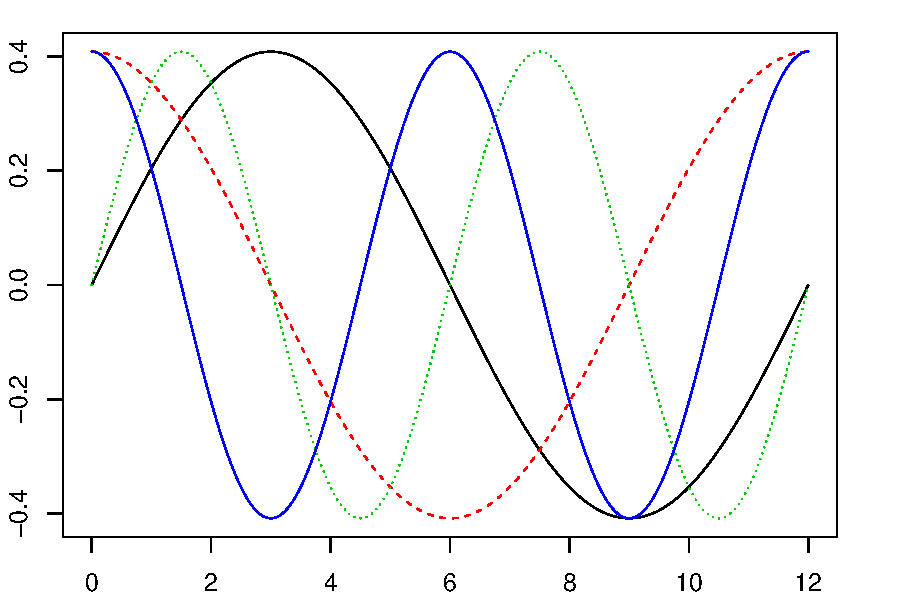
\includegraphics[width=0.8\textwidth]{anexos/base_fourier}
  \caption{Exemplo de base Fourier utilizando 5 funções. Função constante não está representada.}
\end{figure}

\subsubsection*{Base B-splines} \label{sub:Base-B-splines}

Funções spline constituem uma base indicada para quando os dados possuem natureza não-periódica. 
Cada uma das funções $\phi_k$ é um polinômio, de uma ordem $m$ pré-estabelecida. 
Como regra de bolso, escolhe-se o grau do polinômio como duas unidades a mais que o número de vezes que a função será derivada.
A grande diferença entre uma base utilizando splines e uma base polinomial convencional é que cada uma das funções da base spline estará definida apenas para um subintervalo do intervalo $[t_0,t_1]$ no qual  deseja-se aproximar a função $f(t)$.
Os locais em que se dividem o intervalo total são pontos denominados de breakpoints.

A base B-spline é um conjunto específico de funções que são adequadas para fazer a aproximação desejada.
A literatura cita vantagens computacionais em se utilizar uma base B-splines em relação a outras, tanto no tempo de estimação dos coeficientes $\hat{c}_k$ como na disponibilidade de pacotes que o implementam em diversas linguagens e softwares diferentes.
Uma referência para aprofundar mais no estudo de splines pode ser encontrada em \citeonline{de_boor_practical_1978}. Um exemplo de base de B-splines é mostrado na figura~\ref{fig-base-bspline} \todo{ajeitar este link}.
\begin{figure}[h!] \label{fig-base-bspline}
  \centering
    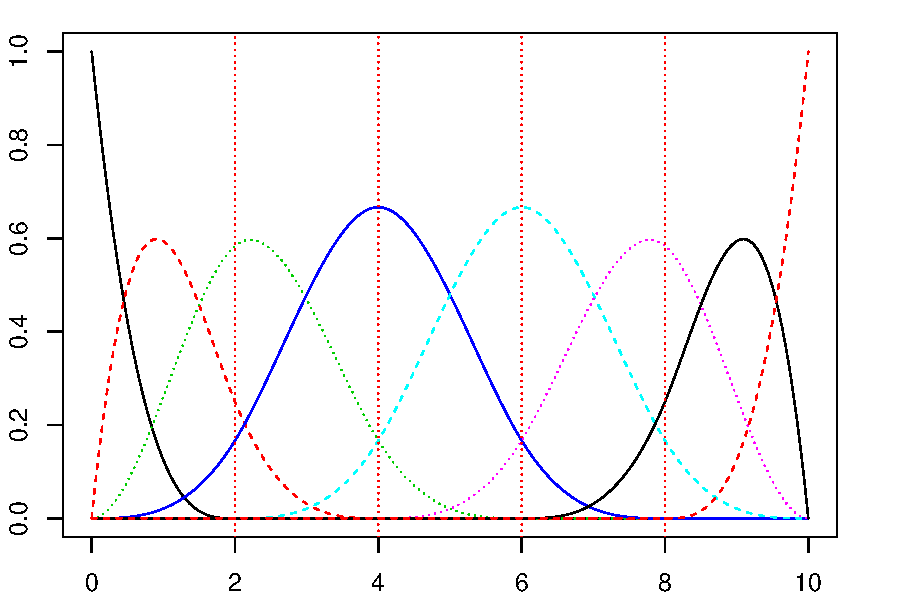
\includegraphics[width=0.8\textwidth]{anexos/base_bsplines1}
  \caption{Exemplo de base B-splines utilizando 10 funções}
\end{figure}

\subsection{Análise de Componente Principal Funcional}
\label{FPCA}

\todo{ajustar} A Análise de Componentes Principais (PCA) é um método muito utilizado na análise de dados multivariados com grandes dimensões, em que o efeito de uma variável, individualmente, não contribui o suficiente para a compreensão dos dados. O método consiste em encontrar os componentes que melhor explicam a variabilidade dos dados. 

A Análise de Componentes Principais Funcionais (FPCA) é uma extensão do método muitivariado para o caso de dados funcionais. 
A FPCA é utilizada, portanto, para reduzir a dimensão de um dado e exibir suas
características mais marcantes de forma mais compreensível e visual. Sendo
$\mathbb{E}(\int\CHI^{2}(t)dt)<\infty$, pelo teorema de Karhunen–Loève é possível igualar uma função a uma soma infinita de funções ortogonais:
\begin{equation}
\CHI(t)=\sum_{k=1}^{\text{\ensuremath{\infty}}}\left(\int\CHI(t)v_{k}(t)dt\right)v_{k},
\end{equation}
em que $v_{1},v_{2},...,$ são as autofunções ortonormais do operador de covariância
\begin{equation}
\Gamma_{\CHI}(s,t)=\mathbb{E}(\CHI(s)\CHI(t))
\end{equation}
associados aos autovalores $\lambda_{1}\geq\lambda_{2}\geq...$ .
Tomando um um número finito de autofunções, temos uma aproximação da função original, representada através das autofunções e seus coeficientes:
\begin{equation}
\tilde{\CHI}^{(q)}=\sum_{k=1}^{\text{\ensuremath{q}}}\left(\int\CHI(t)v_{k}(t)dt\right)v_{k}.
\end{equation}


\subsection{Modelo linear funcional}

Enquanto o modelo linear multivariado inclui um número finito de variáveis explicativas, o caso funcional possui infinitos:
\begin{equation}
Y_{i}=\alpha_{i}+\intop_{0}^{T}\rho(t)\chi_{i}(t)dt+\varepsilon_{i},\label{eq:modelofuncionallinear}
\end{equation}
onde $\alpha$ é o intercepto, $\chi(t)$ é a função que representa
cada dado funcional e $\rho(t)$ o parâmetro único da regressão funcional
paramétrica. O termo $\varepsilon_{i}$ é o termo de erro associado
a cada resposta e que não é explicado pela variável funcional
independente.

A modelagem de dados funcionais, no entanto, requer cuidados adicionais. Pensando no caso multivariado, por exemplo, há um problema quando
o tamanho da amostra é menor do que o número de variáveis explicativas.
Seja
\begin{equation}
Y=X\beta+\varepsilon
\end{equation}
o modelo a ser estimado, se $X$ for uma matriz com o número de linhas
maior que o de colunas, necessariamente haverá variáveis livres. Assim,
diferentes valores de $\beta$ podem ser utilizados para gerar os
mesmos valores de $Y$. Além disso, é muito provável que o espaço
gerado pela matriz $X$ possua uma dimensão maior que a dimensão de
Y, tornando possível encontrar soluções em que $\varepsilon_{i}=0$,
para todo $i$. 

Uma modelagem em que o modelo se ajusta perfeitamente aos dados (denominado
\emph{overfitting}) não é interessante, pois sua variabilidade será
muito alta. Modelos com alta variabilidade possuem capacidade preditiva
pobre, sendo péssimos em generalizar os dados e dando muita ênfase
ao ruído presente. 

Como um dado funcional está avaliado num espaço infinito dimensional,
o modelo apresentado na equação (\ref{eq:modelofuncionallinear})
também possuirá excesso de variáveis explicativas em relação à amostra.
Dessa forma, alguma estratégia deve ser montada para realizar a regularização,
isto é, impedir o \emph{overfitting} de ocorrer. A seguir, duas maneiras
de realizar a regularização serão investigadas: a primeira delas é
restringir a quantidade de funções base para tirar a capacidade de
ajuste perfeito aos dados, e a segunda é atribuir uma penalização
para as flutuações da função modelada.


\subsubsection*{Regularização usando funções base restritas}

Sejam $\theta_{0},\theta_{1},...$ e $\psi_{0},\psi_{1},...$ bases
funcionais escolhidas, de acordo com a seção (\ref{sub:Bases-para-representa}),
e seja $K_{\beta}$ a quantidade de funções base utilizadas em
\begin{equation}
\beta(t)=\sum_{k}^{K_{\beta}}b_{k}\theta_{k}(t)\quad ou\quad\beta=\boldsymbol{\theta'b}
\end{equation}
tal que a perda de informação ao modelar $\beta$ não seja grande
ao se modelar a variável explicativa. Ao mesmo tempo, toma-se $K_{z}$
da mesma forma para que
\begin{equation}
\chi_{i}(t)=\sum_{k}^{K_{z}}c_{ik}\psi_{k}(t)\quad ou\quad\chi(s)=\boldsymbol{C\psi(t)}
\end{equation}
também não tenha grande perda de informação nem \emph{overfitting}.
$C$ é uma matriz $N$ (tamanho da amostra) por $K_{z}$. Assim, o
modelo (\ref{eq:modelofuncionallinear}) pode ser reescrito da seguinte
forma:
\begin{equation}
\hat{Y_{i}}=\intop_{0}^{T}\rho(t)\chi(t)dt=\intop_{0}^{T}\boldsymbol{C}\psi(t)\theta(t)'\boldsymbol{b}\, dt=\boldsymbol{C}\boldsymbol{J}_{\psi\theta}\boldsymbol{b},
\end{equation}
em que $\boldsymbol{J}_{\psi\theta}$ é uma matriz $K_{z}$ por $K_{\beta}$
definida por:
\begin{equation}
\boldsymbol{J}_{\psi\theta}=\int\psi(t)\boldsymbol{\theta}'(t)\, dt.
\end{equation}

\subsubsection*{Regularização com penalização por não-suavidade}

Considere o seguinte problema de minimização dos resíduos quadráticos
penalizado:
\begin{equation}
PENSSE_{\lambda}(\alpha,\beta)=\underbrace{\sum_{i=1}^{N}[y_{i}-\alpha-\int z_{i}(t)\beta(t)dt]^{2}}_{g}+\lambda\underbrace{\int[L\beta(t)]^{2}dt}_{h},\label{eq:pensse}
\end{equation}
em que $L$ é um operador diferencial linear adequado para o problema.
Enquanto $g$ penaliza a distância ao quadrado entre a variável resposta
e a variável real, o $h$ penaliza a falta de suavidade do modelo.
Assim, o parâmetro $\lambda$ irá ponderar o grau de suavização da
curva. Tomando $\lambda=0$, a curva vai se ajustar perfeitamente
aos dados, e haverá um problema de \emph{overfitting}. Por outro lado,
quando $\lambda\rightarrow\infty$, a regressão será uma curva totalmente
suave.

Há duas maneiras de escolher o valor de $\lambda$. A primeira é fazê-lo
de forma subjetiva, isto é, fazendo variar o parâmetro e escolher
a que mais agrade visualmente. A segunda é escolher automaticamente
através de um procedimento de \emph{cross-validation},
realizado da seguinte forma:
\begin{itemize}
\item Obtém-se as estimativas de $\alpha_{\lambda}^{(-i)}$ e $\beta_{\lambda}^{(-i)}$,
obtidas encontrando os valores de $\alpha$ e $\beta$ que minimizam
a equação (\ref{eq:pensse}) de toda a amostra, com exceção dos valores
em $(z_{i},y_{i})$. 
\item Monta-se a função 
\[
CV(\lambda)=\sum_{i=1}^{N}[y_{i}-\alpha_{\lambda}^{(-i)}-\int z_{i}(t)\beta_{\lambda}^{(-i)}(t)dt]^{2}.
\]
Escolhendo $\lambda$ de forma a minimizar a função $CV(\lambda)$
será a escolha ótima do parâmetro utilizando-se o procedimento de
\emph{cross-validation}.
\end{itemize}

\subsection{Séries temporais funcionais}

É possível fazer a modelagem de uma série temporal pela decomposição da série em fatores utilizando FPCA. Seja a série temporal $\{ f_t(\tau) \}_{t=t_1}^{t_2}$ estimada no  intervalo $[t_1,t_2]$. Haverá, portanto, $n=t_2-t_1+1$ funções representando a série temporal:
\begin{equation}
f_{t_1}(\tau), f_{t1+1}(\tau), \dots, f_{t2}(\tau)
\end{equation}
Assim como demonstrado na seção~\ref{FPCA}, cada função pode ser aproximada pela combinação linear das autofunções ortonormais do operador de covariância:
\begin{equation}
\widetilde{f}_s(\tau)=\sum_{i=1}^{m}{ \underbrace{ \left(  \int f_s(\tau)  v_i(\tau)dt \right) }_{\phi_{i,t}} } v_i,
\end{equation}
em que $m$ é o número de 
Tomando $t$ no intervalo $[t_1,t_2]$, tem-se uma série temporal de $\phi_i$ associada a cada autofunção. Essa série, por sua vez, pode ser estimada com algum método univariado tradicional, como ARIMA, passeio aleatório, série temporal exponencial, etc. A partir da estimação, pode-se prever cada um dos $\hat{\phi}_{i,t_2+h}$, para cada horizonte de interesse $h$. A curva prevista $f_{t_2+h}(\tau)$ é obtida quando se somam os produtos das autofunções com seus respectivos coeficientes previstos, isto é:
\begin{equation}
\hat{f}_{t_2+h}(\tau)= \sum_{i=1}^{m}{\hat{\phi}_{i,t_2+h} v_i(\tau) }.
\end{equation}

As séries temporais funcionais foram utilizadas na previsão da ETTJ por \citeonline{shang}, com resultados muito bons. Como é uma abordagem funcional já utilizada na literatura, será implementada para comparação com os resultados obtidos pela estimação com métodos de NP-FDA.

\section{Métodos Não-paramétricos para a Análise de dados funcionais}

Nesta seção, será estudada a metodologia não-paramétrica para análise
de dados funcionais. Ao contrário dos modelos paramétricos, desta
vez não será suposta nenhuma forma funcional para a estimação. Assim,
o modelo tomará a seguinte forma:
\[
Y=r(\chi)+erro,
\]
em que $r(\cdot)$ é um operador linear contínuo de $\mathcal{H}$
em $\mathbb{R}$. A maioria das funções utilizadas para implementação
podem ser encontradas em \emph{http://www.lsp.ups-tlse.fr/staph/npfda. }

\subsection{Funções Kernel}

Para dados funcionais, utiliza-se funções Kernel assimétricas, tais que $\int K = 0$, com suporte compacto em $[0,1]$ (à exceção do Kernel gaussiano, que possui suporte em $[0,\infty)$) e tais que $\forall u \in (0,1), K(u) > 0$. O motivo de se utilizar funções Kernel assimétricas é o fato de as semi-métricas utilizadas para medir a distância entre as curvas produzirem apenas valores positivos. As funções Kernel serão utilizadas pelos métodos estudados a seguir, possuindo uma característica de atribuir peso localmente.

Seja $I_R(u)$ uma função definida como $1$, quando $u \in \mathbb{R}$ e 0, caso contrário, as funções Kernal mais utilizadas são as seguintes:
\begin{description}
	\item[Kernel uniforme] $K(u)= I_{[0,1]}(u)$
    \item[Kernel triangular] $K(u)= 2(1-u)I_{[0,1]}(u)$
    \item[Kernel quadrático] $K(u)= \frac {3}{2} (1 - u^2) I_{[0,1]}(u)$
    \item[Kernel gaussiano] $K(u)= \frac {\sqrt{2}}{\sqrt{\pi}} exp{-\frac{u^2}{2}} I_{[0,\infty]}(u)$
\end{description}

\subsection{Métodos para a previsão}
\label{metodos-previsao-npfda}

Nesta seção, apresenta-se as três formas de se fazer estimações conforme apresentado por \citeonline{vieu_nonparametric_2006}.


\subsubsection*{Previsão via regressão}

Utiliza-se um regressor não linear $r(\chi)=E(Y|\boldsymbol{\chi}=\chi)$
e a previsão por esse método será dada por:
\[
\hat{y}=\hat{r}(\chi).
\]

Para a estimação de $\hat{r}(\chi)$, é proposta a utilização do estimador
não paramétrico utilizando-se uma função kernel assimétrica $K$:~\ref{peso-local}

\begin{equation}
\hat{r}(\chi)=\frac{\sum_{i=1}^{n}Y_{i}K(h^{-1}d(\chi,\boldsymbol{\chi}_{i})}{\sum_{i=1}^{n}K(h^{-1}d(\chi,\CHI_{i})}.
\end{equation}

Assim, para se atribuir pesos localmente, utilizando funções Kernel, pra dados funcionais, define-se:
\begin{equation} \label{peso-local}
\Delta_i=\frac{K(h^{-1}d(\chi,\boldsymbol{\chi}_{i})}{\mathbb{E} \left( K(h^{-1}d(\chi,\CHI_{i}) \right)},
\end{equation}



\subsubsection*{Previsão via função de densidade acumulada condicional}

A estratégia é utilizar a função densidade acumulada condicional

\begin{equation} \label{fd-acum}
F_{Y}^{\CHI}(\chi,y)=E(1_{(-\infty,y]}(Y)|\CHI=\chi).
\end{equation}
A partir da estimação de $F_{Y}^{\CHI}(\chi,y)$, toma-se por estimativa
o valor de $m(\chi)=inf\{y\in\mathbb{R\mid}F_{Y}^{\CHI}(\chi,y)\geq1/2\}$.
Assim, teremos 
\[
\hat{y}=\hat{m}(\chi).
\]
Já $F_{Y}^{\CHI}(\chi,y)$ pode ser estimada da seguinte forma:
\begin{equation}
\hat{F}_{Y}^{\CHI}(\chi,y)=\frac{\sum_{i=1}^{n}K(h^{-1}d(\chi,\boldsymbol{\chi}_{i})H(g^{-1}(y-Y_{i})}{\sum_{i=1}^{n}K(h^{-1}d(\chi,\CHI_{i})},
\end{equation}
onde $H$ é uma função definida por $H(u)=\int_{-\infty}^{u}K_{0}(v)dv$,
e $K_{0}$ é uma função kernel simétrica.
Utilizando-se a mesma função acumulada, é possível também estimar a função condicional quantílica $\hat{t}_{\alpha}(\chi)$, para qualquer $\alpha$ em $[0,1/2]$, bastando para isso tomar
\begin{equation}
\hat{t}_{\alpha}(\chi)=inf\{y\in\mathbb{R},\hat{F}_{Y}^{\CHI}(\chi,y)\geq\alpha
\end{equation}


\subsubsection*{Previsão via moda da função de densidade}

Como a equação \ref{fd-acum} fornece uma expressão para a função de densidade acumulada, é possível utilizar uma outra estratégia para a estimação, baseada na função de densidade. O primeiro passo é, a partir da f.d.a conseguir derivar uma função de densidade. Isto pode ser obtido através da seguinte expressão:
\begin{equation}
\hat{f}_Y^\chi(\chi,Y)=\frac{\partial}{\partial y} \hat{F}_Y^\chi.
\end{equation}
Sendo, então, $H$ diferenciável, temos:
\begin{equation}
\frac{\partial}{\partial y} \hat{F}_{Y}^{\CHI}(\chi,y) = \frac{\sum_{i=1}^{n}K(h^{-1}d(\chi,\boldsymbol{\chi}_{i}) \frac{\partial}{\partial y} H(g^{-1}(y-Y_{i})}{\sum_{i=1}^{n}K(h^{-1}d(\chi,\CHI_{i})},
\end{equation}
o que resulta na expressão final de estimação:
\begin{equation}
\hat{f}_{Y}^{\CHI}(\chi,y) = \frac{\sum_{i=1}^{n}K(h^{-1}d(\chi,\boldsymbol{\chi}_{i}) \frac{1}{g} H'(g^{-1}(y-Y_{i})}{\sum_{i=1}^{n}K(h^{-1}d(\chi,\CHI_{i})}.
\end{equation}

\subsection{Medindo a distância entre as curvas utilizando semi-normas}

Nas seções anteriores, utilizou-se a função $d(\cdot)$ para expressar
a distância entre duas curvas. Medir a distância entre variáveis é
simples quando trabalhamos no espaço $\mathbb{R}^{p}$, sendo $p$
um número finito. Isso ocorre pois há equivalência entre todas as
normas em espaços de dimensões finitas. Podendo-se utilizar, por exemplo,
a norma euclidiana $||\cdot||$%
\footnote{Seja $x=(x_{1},...,x_{p})^{T}$ um vetor pertencente a $\mathbb{R}^{p}$,
então$||x||^{2}=\sum_{j=1}^{p}(x_{j})^{2}=x^{T}x$.%
} . A escolha da norma num modelo multivariado não será uma tarefa
que requer atenção.

Por outro lado, as variáveis funcionais tomam valores num espaço infinito
dimensional. Em espaços dessa dimensionalidade, a equivalência de normas não se
aplica. Além disso, a utilização de uma métrica pode não ser interessante
por ser muito restritiva. Por isso, $d(\cdot)$ será escolhida como
uma semi-norma, dentro de um espaço semi-métrico, ao invés de uma
norma num espaço métrico. As duas gozam das mesmas propriedades, com
exceção de que para a semi-norma vale que $d(x,y)=0\nRightarrow x=y$. 


\subsubsection*{Semi-métrica baseada em Análise de Componente Principal Funcional
(FPCA)}

A FPCA é utilizada para reduzir a dimensão de um dado e exibir suas
características mais marcantes de forma mais compreensível. Sendo
$\mathbb{E}(\int\CHI^{2}(t)dt)<\infty$, podemos reescrever $\CHI$
como a sua expansão pela combinação linear de seus componentes principais:
\begin{equation}
\CHI=\sum_{k=1}^{\text{\ensuremath{\infty}}}\left(\int\CHI(t)v_{k}(t)dt\right)v_{k},
\end{equation}
em que $v_{1},v_{2},...,$ são as autofunções ortonormais do operador de covariância
\begin{equation}
\Gamma_{\CHI}(s,t)=\mathbb{E}(\CHI(s)\CHI(t))
\end{equation}
associados aos autovalores $\lambda_{1}\geq\lambda_{2}\geq...$ .
Tomando um um número finito de autofunções, temos:
\begin{equation}
\tilde{\CHI}^{(q)}=\sum_{k=1}^{\text{\ensuremath{q}}}\left(\int\CHI(t)v_{k}(t)dt\right)v_{k}.
\end{equation}
Dessa forma, é construída uma família de semi-métricas com parâmetro
$q$:
\begin{equation}
d_{q}^{PCA}(\CHI_{i},\chi)=\sqrt{\sum_{k=1}^{\text{\ensuremath{q}}}\left(\int[\CHI_{i}(t)-\chi(t)]v_{k}(t)dt\right)^{2}}
\end{equation}



\subsubsection*{Semi-métrica baseada em derivativas}

É possível construir outra família de semi-métricas a partir da distância
entre seus derivativos, da forma a seguir:
\begin{equation}
d_{q}^{deriv}(\CHI_{i},\chi)=\int\left(\CHI_{i}^{(q)}(t)-\chi^{(q)}(t)\right)^{2}dt,
\end{equation}
onde $\chi^{(q)}(t)$ representa a $q$-ésima derivada de $\chi(t)$.
Para o cálculo da derivativa, primeiro os dados serão expandidos na
base B-splines, conforme mostrado na seção (\ref{sub:Base-B-splines}).
Após, pode-se derivar a função Spline na ordem desejada para calcular
a distância entre $\chi$ e $\CHI_{i}$.

É importante enfatizar que, como foi feita a substituição das funções
$\chi$ e $\CHI_{i}$ por funções Spline $S_{1}(t)$ e $S_{2}(t)$
que as representam, é possível trabalhar com dados desbalanceados,
isto é, cujas observações não foram feitas nos exatos mesmos pontos
de $t$. No entanto, salienta-se que o método de representação de
uma função $f(t)$ por meio de uma função Spline $S(t)$ funciona
bem quando $f(t)$ é uma função suave.


%-----------------------
% Metodologia
%-----------------------

\chapter{Metodologia}

Para a realização das estimações da ETTJ, os métodos utilizados serão os mesmos dos apresentados na revisão de literatura, tanto para o caso paramétrico quanto para o não-paramétrico. Assim, o estudo será relativamente abrangente em relação à adequação da abordagem funcional para a modelagem do problema em questão.

Como estratégia de avaliação, os métodos de estimação serão aplicados a apenas uma parte da amostra, e a previsão é feita fora da amostra utilizada para fazer a estimação o restante para ser utilizado como teste da capacidade de previsão. Assim, pode-se calcular o Erro Quadrático Médio (EQM) das previsões e comparar suas performances. 

\subsection*{Dados}

Os dados utilizados serão dados diários (no período de 25/11/1985 até 09/02/2012, constituindo 6537 dias) da taxa de juros para títulos de maturidades diversas (mensais no intervalo de 1 mês até 30 meses). Assim, a base de dados contém 196110 observações. A figura~\ref{fig-est-termo} contém as séries temporais das diferentes maturidades.
\begin{figure}[h!] \label{fig-est-termo}
  \centering
    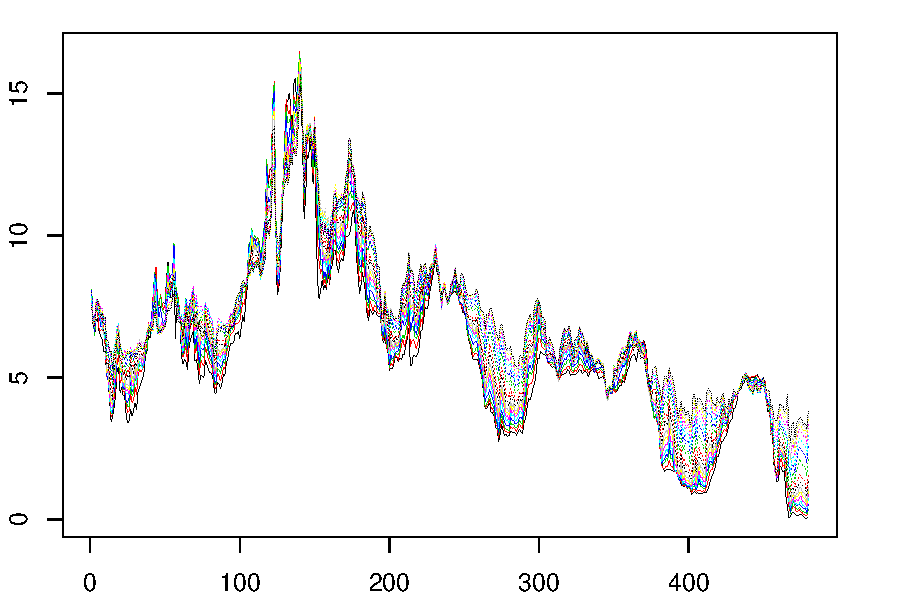
\includegraphics[width=0.8\textwidth]{anexos/taxas_juro}
  \caption{Estrutura a termo da taxa de juros}
\end{figure}

Trabalha-se com uma base constituída de x \todo{completar as maturidades e observações} maturidades e y observações dessas maturidades. Como se está interessado na previsão dos valores da taxa de juros fora da amostra, este trabvalho modela cada dado funcional como uma observação no tempo $t$ de $f_t(\tau)$. A função $f_t:[\tau_1,\tau_k] \rightarrow \mathbb{R}$ é construída com base nos valores discretos ${\tau_1, ..., \tau_k}$, em que $k$ é o número total de maturidades.



\subsection*{Implementação}

A implementação será feita em R, uma linguagem de programação construída dentro da lógica de software livre. Ela é usada predominantemente para solucionar problemas estatísticos. Por ser livre, é amplamente incrementada por pesquisadores, possuindo um enorme banco de funções e pacotes. Mais sobre a linguagem R pode ser obtido em http://cran.r-project.org/. O ambiente de programação que será utilizado é o software RStudio, também um programa de código aberto.

Para cada valor previsto, estima-se o modelo em uma dada janela num intervalo $[t_a,t_b]$, e prevê-se o valor de  $\hat{y}_{t+h|t}(\tau_i)$, em que $h$ é o horizonte da previsão e $\tau_i$ o valor da maturidade. Assim, para cada valor previsto, utiliza-se uma janela que termina $h$ unidades de tempo anteriores à previsão.

Dois tipos de janela móvel foram utilizados: com tamanho fixo e tamanho expandível. 
No primeiro tipo, a janela de estimação possui tamanho fixo. Então, enquanto utiliza-se a janela $[t_a,t_b]$ para estimar o modelo e fazer a previsão do valor de $\hat{y}_{t+h|t}(\tau_i)$, a janela $[t_{a+1},t_{b+1}]$ é utilizada para prever o valor de $\hat{y}_{t+1+h|t+1}(\tau_i)$. Quando trabalha-se com tamanho expandível, o ponto de início do intervalo se mantém, mas o final dele é incrementado: utilizam-se os intervalos $[t_{a},t_{b}] ,[t_{a},t_{b+1}],[t_{a},t_{b+2}],\dots$  pra prever $\hat{y}_{t+h|t}(\tau_i),\hat{y}_{t+1+h|t}(\tau_i),\hat{y}_{t+2+h|t}(\tau_i),\dots$, respectivamente.

Quando se trabalha com tamanho expandível, obtém-se o aproveitamento máximo dos dados disponíveis para efetuar a previsão, já que todo valor conhecido pode ser utilizado, enquanto quando trabalha-se com janela fixa, a parte inicial da amostra vai sendo descartada à medida que a janela avança. Ter mais dados é essencialmente importante quando se utiliza métodos cuja convergência dos parâmetros aos seus valores verdadeiros é mais lenta, como ocorre normalmente com os métodos não-paramétricos. 

A vantagem de trabalhar com janela móvel e tamanho fixo, por outro lado, é que oferece resultados mais robustos, em que o ponto de início da série de dados não influencia a previsão de determinado valor. É possível verificar em quais subintervalos da série o método possui capacidade melhor de previsão, sem confundir o efeito do período de previsão com o efeito de aumento da quantidade de dados janela.

\section{Previsão com os Métodos escolhidos como \emph{benchmark}}

Para melhor avaliar os resultados dos métodos investigados neste trabalho, compara-se a capadidade de previsão deles com outros métodos utilizados na literatura. São eles: o modelo de DL, o passeio aleatório e o modelo AR(1).

\subsection{Previsão com Método de Diebold-Li}

Seja o modelo de \citeonline{diebold_forecasting_2006} a seguir:

$$y_{t}(\tau)=\beta_{1,t}+\beta_{2,t}\left( \frac { 1-e^{ -\lambda \tau  } }{ \lambda\tau}  \right) -\beta_{3,t}\left( \frac { 1-e^{ -\lambda \tau  } }{ \lambda \tau  } -e^{ -\lambda \tau  } \right),$$
o primeiro passo para realizar as previsões é definir o valor de $\lambda$, que é mantido fixo durante a estimação, ao contrário de quando se utiliza o modelo de NS. 

Para escolher o valor de $\lambda$ emprega-se um método de \emph{cross-validation}. A busca foi realizada tomando valores dentro do intervalo $[0.2,1.2]$, com incrementos de $0.05$. O intervalo de aprendizado foi dividido em duas partes: uma para estimar (contendo 60\% do intervalo) e outra para prever fora da amostra (contendo o resto). Assim, para cada um dos valores testados, as previsões foram feitas e o Erro Quadrático Médio calculado. 
De acordo com as simulações executadas nesse trabalho, tomar $\lambda=0.5$ gerou as melhores previsões dentro do intervalo de aprendizagem.

Uma vez fixo o valor de $\lambda$, pode-se partir para as estimações por completo. Para cada período de $t$, os valores de $\hat{\beta}_{1,t}$, $\hat{\beta}_{2,t}$ e $\hat{\beta}_{3,t}$ são estimadas em \emph{cross-section}.

A partir dos valores de  $\hat{\beta_1}$, $\hat{\beta_2}$ e $\hat{\beta_3}$, pode-se recriar a curva de juros, para um vetor qualquer de maturidades, utilizando-se a função . Note que os $\beta$'s podem reproduzir quaisquer maturidades desejadas, inclusive aquelas que não foram utilizadas estimar os $\beta$'s.

Com base nos valores de $\hat{\beta}$ já estimados, prevê-se os valores futuros de $\hat{\beta}$ através de um modelo AR(1), com $h$ passos à frente. 
$$\hat{\beta} _{ t+h/t } = \hat{c} + \hat{\Gamma}\hat{\beta}_t$$
Após, o valor previsto para cada maturidade é obtido após multiplicar $\beta$ pelos fatores.
$$\hat { y } _{ t+h/t }(\tau)=\hat{\beta} _{ 1,t+h/t }+\hat{\beta} _{ 2,t+h/t }\left( \frac { 1-e^{ -\lambda \tau  } }{ \lambda \tau  }  \right) -\hat{\beta} _{ 3,t+h/t }\left( \frac { 1-e^{ -\lambda \tau  } }{ \lambda \tau  } -e^{ -\lambda \tau  } \right)$$


\subsection{Passeio aleatório}
Considera-se a série temporal um passeio aleatório. Assim, para cada qualquer horizonte, considera-se que o valor futuro da maturidade se manterá o mesmo:

\begin{equation}
\hat{y}_{t+h/t}(\tau_i)=y_t(\tau_i).
\end{equation}


\subsection{AR(1)}
Ajusta-se, à cada maturidade da curvas de juros, um modelo auto-regressivo de ordem 1, utilizando mínimos quadráticos ordinários:
$$y_t(\tau_i)=\alpha(\tau_i) + \phi(\tau_i) y_{t-1}(\tau_i)+\varepsilon_{t}(\tau_i).$$
Assim, minimizando os valores quadráticos de $\varepsilon$ obtém-se os estimadores de $\alpha(\tau_i)$ e $\phi(\tau_i)$.
Pode-se, então, fazer a estimação $1$ passo à frente utilizando os valores dos coeficientes estimados na equação do modelo:
\begin{equation}
\hat{y}_{t+1/t}(\tau_i)=\hat{\alpha}(\tau_i) + \hat{\phi}(\tau_i) y_t(\tau_i).
\end{equation}

Para prever mais do que $1$ passo à frente, é possível utilizar o valor previsto para prever outro passo à frente:
\begin{equation}
\hat{y}_{t+p/t}(\tau_i)=\hat{\alpha}(\tau_i) + \hat{\phi}(\tau_i) \hat{y}_{t+p-1/t}(\tau_i),
\end{equation}
e assim por diante. Iterativamente, consegue-se então utilizar o método para fazer a previsão $n$ passos à frente.

\section{Previsão com Métodos não-paramétricos para FDA}

Seja $(\chi_i,Y_i)_{i=t_i,...,t_f}$ pares de variáveis aleatórias funcionais identicamente distribuídos como $(\CHI,\boldsymbol{Y})$, tomando valor em $E \times \mathbb{R}$, em que $(E,d)$ é um espaço semi-métrico. O objetivo do problema é prever a resposta escalar de um preditor funcional $\chi$ utilizando algum dos três métodos apresentados na seção \ref{metodos-previsao-npfda}. Como a resposta escalar é uma variável unidimensional, e deseja-se fazer a previsão para diversas maturidades, é necessário fazer a estimação para cada uma das maturidades que se deseja realizar previsões.

Como entrada do problema, há $m$ séries temporais de tamanho $n$, uma para cada maturidade disponível. Outra forma de se enxergar a base de dados é através de uma matriz $Y_{m \times n}$, conforme mostra-se a seguir:
\begin{equation} 
Y_{m,n} = 
 \begin{bmatrix}
	  y_{1,1} & y_{1,2} & \cdots & y_{1,n} \\
	  y_{2,1} & y_{2,2} & \cdots & y_{2,n} \\
	  \vdots  & \vdots  & \ddots & \vdots  \\
	  y_{m,1} & y_{m,2} & \cdots & y_{m,n}
 \end{bmatrix}
\end{equation}
Assim, sendo $[t_a,t_b]$ o intervalo para estimação e $h$ o horizonte para previsão desejado, uma  curva $\chi_t(\tau)$ pertencente à amostra é formada pela sequência dos valores discretos das colunas de $Y$: $(y_{1,t},y_{2,t}, ... , y_{m,t})$. A resposta escalar associada a esta curva de índice $i$ é $y_{\tau_i,t + h}$, levando em conta que se está fazendo previsão para o horizonte $h$ e maturidade $\tau_i$. A amostra inicial é composta dos pares $(\chi_t,y_{\tau,t+h})_{t=t_a,...,t_b-h}$. Para a previsão do valor de $y_{t_b+h}$, toma-se $E(Y|\CHI=\chi)$. 

Uma análise preliminar mostrou que, caso a estimação fosse feita sem nenhum tratamento aos dados, os resultados seriam insatisfatórios. Isto ocorre pois o nível da curva é um dos fatores mais significativos para prever os valores futuros da taxa de juros (uma das razões pelas quais, embora muito simples, o passeio aleatório ainda é um método tido como \emph{benchmark} em trabalhos de previsão de curvas de juros). Assim, a matriz $D$ formada pelas distâncias entre curvas $d(\chi_i,\chi_j)$ possuirá valores mais altos, no geral. Como o fator mais decisivo para a proximidade passa a ser o nível das curvas, perde-se a maior vantagem em utilizar métodos funcionais, que é justamente levar em consideração o formato da função.

Por essa razão, decidiu-se retirar o nível da curva para testar o método. Isto, porém, levanta outra questâo: qual é o valor que representa o nível da curva? A média, alguma maturidade, ou ainda outro valor? Levando isso em conta, considera-se um modelo mais geral de estimação, apresentado a seguir:
\begin{equation}
\hat{y}_{\tau,t+h} - k_t = m(\chi - k_t),
\end{equation}
em que $k \in \mathbb{R}$. Caso $k=0$, tem-se o modelo padrão
\begin{equation}
\hat{y}_{\tau,t+h}= m(\chi),
\end{equation}
e quando $k_t = y_{\tau,t}$, tem-se o modelo de estimação em diferença
\begin{equation}
\Delta \hat{y}_{\tau,t+h}= m(\chi - y_{\tau,t}).
\end{equation}

Além desses valores, achou-se interessante utilizar também outros valores, como tomar $k = \hat{\beta}_{1,t}$, em que $\hat{\beta}_{1,t}$ representa a estimação do primeiro fator no modelo de \citeonline{diebold_forecasting_2006}. 
\todo[inline]{valores retirados}

\subsection*{Escolha da \emph{bandwidth}}

A escolha do valor da \bw é um fator central na estatística não-paramétrica, já que atua é o elemento principal que atua na suavização da função estimada, possuindo um papel de maior impacto que o da função Kernel. É uma escolha delicada, pois se a variância do modelo for muito alta, o poder de previsão será ruim. No outro extremo, se a suavização for máxima, o modelo estimado será um modelo linear, perdendo características importantes dos dados.

\todo[inline]{implicações de h, p. 56}

Há duas formas de definir a \bw: utilizando um valor fixo de $h$, ou definindo uma quantidade fixa de curvas para se levar em conta. A seguir, essas duas formas serão apresentadas.

\begin{itemize}

\item Utilização de \bw \,fixa:

Trabalha-se com um valor único para $h$, independente da curva $\chi$ que deseja-se estimar na regressão. Seja a estimação da seguinte forma:
\[
R_{CV}^{kernel}(x)=\dfrac{\sum_{i=1}^{n}y_{i}K(d_{q}(\boldsymbol{x},\boldsymbol{x_{i}})/h_{opt})}{\sum_{i=1}^{n}K(d_{q}(\boldsymbol{x},\boldsymbol{x_{i}})/h_{opt})},
\]
o valor ótimo para $h_{opt}$ será obtido com base num processo de \emph{cross-validation}. Serão testados valores para $h$ dentro do intervalo $[p(5\%),p(50\%)]$, em que $p(\bullet)$ representa o percentil indicado das distâncias entre pares de curvas $d_q(\boldsymbol{x_j},\boldsymbol{x_i})$. Assim, toma-se 
\[h_{opt} = \operatorname*{arg\,min}_h CV(h),\]
onde 
\[
CV(h) = \sum \limits_{i=1}^n \left(  y_i - R_{(-i)}^{kernel}(\boldsymbol{x}_i)  \right)^2, 
\]
com
\[
R_{-i}^{kernel}(x)=\dfrac{\sum \limits_{j=1,i \neq j}^{n}y_{j}K(d_{q}(\boldsymbol{x},\boldsymbol{x_{j}})/h)}{\sum \limits_{j=1,i \neq j}^{n}K(d_{q}(\boldsymbol{x},\boldsymbol{x_{i}})/h_{opt})}.
\]

\item Vizinhos mais próximos

\todo[inline]{Escrever seção}

\end{itemize}


\section{Metodologia para avaliação da performance das previsões}

As previsões serão avaliadas utilizando as seguintes métricas:

\begin{description}
	\item[Raiz do Erro Quadrático Médio] O erro quadrático médio das previsões é um critério estatístico amplamente utilizado na literatura. Pelo erro ser elevado ao quadrado, esse critério pune com mais severamente os desvios grandes da meta. Ele é obtido pela seguinte expressão: \[ REQM_m(\tau_i) = \sqrt{ \frac{1}{R} \sum _{t = 1}^R (\hat{y}_{t+h|t,m}(\tau_i) - y_{t+h}(\tau_i))^2 } \]
	\item[Erro Quadrático Acumulado de Previsão] É uma metodologia que não fornece um simples indicador comparativo de performance, mas sim um gráfico do comportamento da previsão do método avaliado com relação a algum outro método que é utilizado como \emph{benchmark}. A fórmula para implementar o método é a seguinte:
	\[ EQAP_{m}(\tau_i) = \sum_{t=w+1}^T  \left[ \left( \hat{y}_{t+h|t,benchmark}(\tau_i) - y_{t+h}(\tau_i) \right)^2 - \left( \hat{y}_{t+h|t,m}(\tau_i) - y_{t+h}(\tau_i) \right)^2 \right]. \]
Assim, o trecho em que o gráfico possui inclinação positiva é onde o método avaliado possui performance superior ao \emph{benchmark}, enquanto quando é negativamente inclinado é o método \emph{benchmark} quem possui a melhor performance.
	
	\item[Significância da diferença de previsão]
	
	Giacomini-White e Diebold-Mariano

Embora alguns métodos possuam resultados melhores, em termos de erro quadrático médio, do que outros, é importante saber o quão melhor um método é e se o resultado e estatisticamente importante. 
Para isso,utiliza-se neste trabalho dois testes comumente empregados na literatura para comparar previsões: o teste de 
Giacomini-White (GW) e o teste de Diebold-Mariano (DM).

GW produz uma estatística sobre a significância da diferença de performance de dois métodos de previsão, supondo que estes são 
produzidos a partir de uma janela móvel. A hipótese nula do teste é que os dois métodos comparados, um dado método $m$ e o método \bm, possuem igual capacidade de previsão:
\begin{equation}
\mathbb{H}_0:E[d_{a,t+h}|\delta_{m,t}]=0,
\end{equation}
em que $\delta^{m,t}$ é um vetor $p \times 1$ de funções teste ou instrumentos, $h$ o horizonte de previsão, e 

	
\begin{equation}
GW_{m,n} = n \left( n^{-1} \sum_{t=w+1}^{n-h} \delta_{m,t} d_{m,t+h} \right)' \hat{\Omega}_n^{-1}	
\left( n^{-1} \sum_{t=w+1}^{n-h} \delta_{m,t} d_{m,t+h} \right) \overset{d}{\longrightarrow} \chi_{dim(\delta)}^2
\end{equation}		
	
	\todo[inline]{escrever seção}
	
\end{description}


%---------------------------------
% Resultados
%---------------------------------
\chapter{Resultados}

% ----------------------------------------------------------
% PARTE
% ----------------------------------------------------------
%\part{Preparação da pesquisa}
% ----------------------------------------------------------

% ---
% Capitulo com exemplos de comandos inseridos de arquivo externo 
% ---
%\include{abntex2-modelo-include-comandos}
% ---


% ----------------------------------------------------------
% PARTE
% ----------------------------------------------------------
%\part{Resultados}
% ----------------------------------------------------------

% ---
% primeiro capitulo de Resultados
% ---
%\chapter{Resultados}

% ----------------------------------------------------------
% Finaliza a parte no bookmark do PDF
% para que se inicie o bookmark na raiz
% e adiciona espaço de parte no Sumário
% ----------------------------------------------------------
%\phantompart

% ---
% Conclusão (outro exemplo de capítulo sem numeração e presente no sumário)
% ---
%\chapter*[Conclusão]{Conclusão}
%\addcontentsline{toc}{chapter}{Conclusão}
% ---

%Blau blau blau

% ----------------------------------------------------------
% ELEMENTOS PÓS-TEXTUAIS
% ----------------------------------------------------------
%\postextual
% ----------------------------------------------------------

% ----------------------------------------------------------
% Referências bibliográficas
% ----------------------------------------------------------
\bibliography{Bibliografia-dissertacao}

% ----------------------------------------------------------
% Glossário
% ----------------------------------------------------------
%
% Consulte o manual da classe abntex2 para orientações sobre o glossário.
%
%\glossary

% ----------------------------------------------------------
% Apêndices
% ----------------------------------------------------------

% ---
% Inicia os apêndices
% ---
%\begin{apendicesenv}
%
%% Imprime uma página indicando o início dos apêndices
%\partapendices
%
%\chapter{Tabelas}
%% ----------- movel horizonte 1 ------------------%
%\newgeometry{left=1cm,right=1cm,bottom=1cm}
%
%
%%\begin{landscape}
%Móvel Horizonte 1
%\begin{table}[ht]
%\centering
%\scalebox{0.7}{
%% latex table generated in R 3.0.3 by xtable 1.7-1 package
% Tue Apr 22 13:54:58 2014
\begin{tabular}{rrrrrrrrrrrrrrrrrr}
  \hline
 & 0.25 & 0.5 & 0.75 & 1 & 1.25 & 1.5 & 1.75 & 2 & 2.5 & 3 & 4 & 5 & 6 & 7 & 8 & 9 & 10 \\ 
  \hline
ar & 1.01 & 1.00 & 1.01 & 1.01 & 1.01 & 1.01 & 1.01 & 1.01 & 1.01 & 1.01 & 1.01 & 1.01 & 1.01 & 1.01 & 1.01 & 1.01 & 1.01 \\ 
  crt.d1 & 3.95 & 4.01 & 3.82 & 3.67 & 3.63 & 3.57 & 3.51 & 3.43 & 3.34 & 3.28 & 3.22 & 3.33 & 3.39 & 3.45 & 3.42 & 3.56 & 3.46 \\ 
  crt.d1.rb1 & 1.80 & 1.85 & 1.79 & 1.73 & 1.73 & 1.70 & 1.69 & 1.66 & 1.62 & 1.57 & 1.53 & 1.48 & 1.48 & 1.39 & 1.38 & 1.40 & 1.32 \\ 
  crt.d1.rmat1 & 0.95 & 1.02 & 1.07 & 1.10 & 1.13 & 1.15 & 1.19 & 1.19 & 1.20 & 1.18 & 1.18 & 1.21 & 1.22 & 1.25 & 1.25 & 1.28 & 1.29 \\ 
  crt.d1.rmat17 & 1.31 & 1.33 & 1.30 & 1.27 & 1.28 & 1.26 & 1.27 & 1.25 & 1.23 & 1.20 & 1.18 & 1.15 & 1.17 & 1.09 & 1.09 & 1.09 & 1.02 \\ 
  crt.d1.rmat6 & 0.97 & 0.98 & 1.02 & 1.02 & 1.02 & 1.03 & 1.07 & 1.08 & 1.10 & 1.09 & 1.09 & 1.11 & 1.12 & 1.14 & 1.16 & 1.19 & 1.20 \\ 
  crt.d1.rmean & 1.03 & 1.05 & 1.06 & 1.06 & 1.07 & 1.07 & 1.09 & 1.09 & 1.09 & 1.07 & 1.08 & 1.07 & 1.08 & 1.06 & 1.08 & 1.10 & 1.10 \\ 
  crt.d1.rpmat & 0.95 & 1.01 & 1.04 & 1.05 & 1.09 & 1.08 & 1.09 & 1.09 & 1.06 & 1.04 & 1.04 & 1.04 & 1.07 & 1.02 & 1.02 & 1.05 & 1.02 \\ 
  crt.p1.rpmat & 1.03 & 1.02 & 1.03 & 1.04 & 1.04 & 1.05 & 1.05 & 1.04 & 1.02 & 1.02 & 1.02 & 1.02 & 1.02 & 1.02 & 1.02 & 1.04 & 1.05 \\ 
  crt.p5 & 1.34 & 1.35 & 1.38 & 1.37 & 1.39 & 1.40 & 1.42 & 1.43 & 1.40 & 1.38 & 1.38 & 1.38 & 1.42 & 1.39 & 1.38 & 1.43 & 1.36 \\ 
  crt.p5.rb1 & 1.33 & 1.30 & 1.25 & 1.23 & 1.25 & 1.25 & 1.26 & 1.26 & 1.25 & 1.23 & 1.25 & 1.23 & 1.26 & 1.21 & 1.20 & 1.21 & 1.16 \\ 
  crt.p5.rmat1 & 0.97 & 1.11 & 1.16 & 1.15 & 1.15 & 1.15 & 1.18 & 1.20 & 1.17 & 1.16 & 1.16 & 1.15 & 1.17 & 1.16 & 1.18 & 1.21 & 1.21 \\ 
  crt.p5.rmat17 & 1.09 & 1.05 & 1.09 & 1.09 & 1.12 & 1.13 & 1.16 & 1.18 & 1.18 & 1.16 & 1.17 & 1.14 & 1.16 & 1.09 & 1.09 & 1.10 & 1.02 \\ 
  crt.p5.rmat6 & 1.02 & 1.00 & 1.02 & 1.00 & 1.00 & 1.02 & 1.05 & 1.08 & 1.08 & 1.07 & 1.09 & 1.08 & 1.10 & 1.09 & 1.12 & 1.16 & 1.15 \\ 
  crt.p5.rmean & 0.99 & 1.00 & 1.03 & 1.02 & 1.05 & 1.06 & 1.09 & 1.11 & 1.09 & 1.06 & 1.06 & 1.04 & 1.07 & 1.06 & 1.07 & 1.10 & 1.09 \\ 
  crt.p5.rpmat & 0.97 & 1.03 & 1.02 & 1.02 & 1.04 & 1.03 & 1.04 & 1.05 & 1.03 & 1.03 & 1.07 & 1.14 & 1.16 & 1.13 & 1.07 & 1.06 & 1.04 \\ 
  diebold.02 & 1.15 & 1.01 & 1.03 & 1.03 & 1.03 & 1.02 & 1.02 & 1.02 & 1.01 & 1.02 & 1.02 & 1.02 & 1.02 & 1.02 & 1.02 & 1.02 & 1.02 \\ 
  diebold.05 & 1.08 & 0.97 & 1.01 & 1.02 & 1.03 & 1.03 & 1.03 & 1.04 & 1.04 & 1.03 & 1.02 & 1.02 & 1.02 & 1.02 & 1.01 & 1.02 & 1.02 \\ 
  ftsa.p1\_arima & 2.24 & 2.00 & 1.66 & 1.46 & 1.30 & 1.17 & 1.09 & 1.06 & 1.06 & 1.12 & 1.34 & 1.57 & 1.80 & 1.96 & 2.08 & 2.27 & 2.31 \\ 
  ftsa.p2\_arima & 1.33 & 1.07 & 0.99 & 0.99 & 1.02 & 1.03 & 1.05 & 1.06 & 1.04 & 1.02 & 1.02 & 1.02 & 1.06 & 1.05 & 1.08 & 1.13 & 1.12 \\ 
  ftsa.p2\_arima.rb1 & 1.10 & 1.02 & 1.02 & 0.99 & 1.00 & 1.01 & 1.03 & 1.04 & 1.02 & 1.01 & 1.02 & 1.00 & 1.02 & 0.99 & 0.99 & 1.02 & 0.99 \\ 
  ftsa.p2\_arima.rmat1 & 1.00 & 1.02 & 1.03 & 1.01 & 1.03 & 1.04 & 1.05 & 1.06 & 1.06 & 1.05 & 1.05 & 1.04 & 1.05 & 1.03 & 1.04 & 1.08 & 1.09 \\ 
  ftsa.p3\_arima & 1.08 & 1.01 & 0.99 & 0.98 & 1.01 & 1.02 & 1.04 & 1.04 & 1.03 & 1.02 & 1.03 & 1.02 & 1.04 & 1.03 & 1.03 & 1.07 & 1.05 \\ 
  ftsa.p3\_ets & 1.00 & 0.91 & 0.92 & 0.93 & 0.96 & 0.98 & 1.01 & 1.02 & 1.02 & 1.01 & 1.03 & 1.02 & 1.04 & 1.02 & 1.03 & 1.07 & 1.05 \\ 
  ftsa.p3\_ets.rmat17 & 0.91 & 0.92 & 0.95 & 0.96 & 0.98 & 0.99 & 1.01 & 1.02 & 1.01 & 1.00 & 1.00 & 0.99 & 1.00 & 0.99 & 1.00 & 1.04 & 1.00 \\ 
  ftsa.p5\_arima & 0.96 & 0.99 & 0.97 & 1.03 & 1.09 & 1.07 & 1.05 & 1.04 & 0.99 & 0.98 & 1.00 & 1.02 & 1.04 & 1.04 & 1.04 & 1.07 & 1.04 \\ 
  ftsa.p5\_arima.rb1 & 1.00 & 1.03 & 1.01 & 1.08 & 1.04 & 1.03 & 1.03 & 1.03 & 1.02 & 1.01 & 1.01 & 1.03 & 1.06 & 1.02 & 1.01 & 1.02 & 0.99 \\ 
  ftsa.p5\_arima.rmat1 & 1.00 & 1.01 & 1.00 & 0.99 & 1.03 & 1.04 & 1.05 & 1.06 & 1.04 & 1.03 & 1.03 & 1.03 & 1.04 & 1.04 & 1.04 & 1.06 & 1.04 \\ 
  ftsa.p5\_arima.rmat7 & 0.92 & 0.91 & 0.94 & 0.95 & 0.97 & 0.99 & 1.00 & 1.01 & 1.02 & 1.01 & 1.02 & 1.02 & 1.03 & 1.02 & 1.03 & 1.06 & 1.04 \\ 
  ftsa.p5\_ets.rb1 & 0.90 & 0.99 & 0.97 & 1.09 & 1.06 & 1.05 & 1.03 & 1.03 & 1.01 & 1.00 & 1.01 & 1.05 & 1.08 & 1.04 & 1.02 & 1.03 & 0.99 \\ 
  ftsa.p5\_ets.rmat1 & 1.00 & 1.00 & 1.00 & 0.99 & 1.03 & 1.03 & 1.05 & 1.05 & 1.03 & 1.02 & 1.02 & 1.03 & 1.04 & 1.03 & 1.04 & 1.06 & 1.03 \\ 
  ftsa.p5\_ets.rmat7 & 0.90 & 0.91 & 0.94 & 0.96 & 0.98 & 0.99 & 1.00 & 1.01 & 1.02 & 1.01 & 1.02 & 1.02 & 1.05 & 1.04 & 1.05 & 1.07 & 1.04 \\ 
  ftsa.p5\_rw & 0.94 & 0.98 & 0.97 & 1.03 & 1.10 & 1.08 & 1.07 & 1.06 & 1.01 & 1.00 & 1.01 & 1.03 & 1.05 & 1.05 & 1.04 & 1.07 & 1.04 \\ 
  ftsa.p5\_rw.rmat7 & 0.90 & 0.92 & 0.95 & 0.96 & 0.98 & 0.99 & 1.00 & 1.01 & 1.02 & 1.01 & 1.02 & 1.02 & 1.04 & 1.04 & 1.05 & 1.07 & 1.04 \\ 
  ftsa.p5\_rw.rmean & 0.94 & 0.97 & 0.98 & 0.99 & 1.00 & 1.01 & 1.02 & 1.03 & 1.02 & 1.01 & 1.01 & 1.01 & 1.02 & 1.02 & 1.03 & 1.04 & 1.03 \\ 
   \hline
\end{tabular}
%\caption{Janela móvel - horizonte 1}

%}
%\end{table}
%%\end{landscape}
%\restoregeometry
%
%% ----------- movel horizonte 3 ------------------%
%\newgeometry{left=1cm,right=1cm}
%\begin{landscape}
%Móvel Horizonte 3
%\begin{table}[ht]
%\centering
%\scalebox{0.9}{
%% latex table generated in R 3.0.3 by xtable 1.7-1 package
% Tue Apr 22 13:54:59 2014
\begin{tabular}{rrrrrrrrrrrrrrrrrr}
  \hline
 & 0.25 & 0.5 & 0.75 & 1 & 1.25 & 1.5 & 1.75 & 2 & 2.5 & 3 & 4 & 5 & 6 & 7 & 8 & 9 & 10 \\ 
  \hline
ar & 1.01 & 1.01 & 1.01 & 1.00 & 1.01 & 1.01 & 1.01 & 1.01 & 1.01 & 1.01 & 1.01 & 1.01 & 1.02 & 1.02 & 1.02 & 1.02 & 1.01 \\ 
  crt.d1 & 2.34 & 2.29 & 2.22 & 2.20 & 2.22 & 2.21 & 2.20 & 2.18 & 2.16 & 2.16 & 2.20 & 2.28 & 2.36 & 2.44 & 2.44 & 2.50 & 2.54 \\ 
  crt.d1.rb1 & 1.31 & 1.35 & 1.35 & 1.35 & 1.36 & 1.37 & 1.37 & 1.37 & 1.34 & 1.32 & 1.30 & 1.30 & 1.28 & 1.26 & 1.24 & 1.23 & 1.21 \\ 
  crt.d1.rmat1 & 0.99 & 1.06 & 1.11 & 1.12 & 1.15 & 1.17 & 1.19 & 1.20 & 1.19 & 1.17 & 1.18 & 1.20 & 1.20 & 1.21 & 1.21 & 1.22 & 1.25 \\ 
  crt.d1.rmat17 & 1.07 & 1.12 & 1.15 & 1.15 & 1.17 & 1.18 & 1.19 & 1.19 & 1.18 & 1.16 & 1.15 & 1.14 & 1.13 & 1.12 & 1.10 & 1.10 & 1.09 \\ 
  crt.d1.rmat6 & 0.93 & 1.00 & 1.05 & 1.06 & 1.09 & 1.11 & 1.13 & 1.14 & 1.13 & 1.11 & 1.12 & 1.14 & 1.14 & 1.15 & 1.15 & 1.16 & 1.19 \\ 
  crt.d1.rmean & 0.96 & 1.03 & 1.07 & 1.08 & 1.11 & 1.12 & 1.14 & 1.14 & 1.13 & 1.12 & 1.11 & 1.12 & 1.12 & 1.12 & 1.12 & 1.12 & 1.14 \\ 
  crt.d1.rpmat & 0.99 & 1.04 & 1.07 & 1.09 & 1.10 & 1.11 & 1.11 & 1.12 & 1.11 & 1.11 & 1.11 & 1.11 & 1.10 & 1.10 & 1.10 & 1.09 & 1.09 \\ 
  crt.p1.rpmat & 1.05 & 1.07 & 1.10 & 1.16 & 1.17 & 1.19 & 1.18 & 1.19 & 1.13 & 1.08 & 1.08 & 1.08 & 1.09 & 1.10 & 1.10 & 1.12 & 1.10 \\ 
  crt.p5 & 1.12 & 1.21 & 1.24 & 1.26 & 1.28 & 1.29 & 1.30 & 1.30 & 1.28 & 1.28 & 1.28 & 1.31 & 1.33 & 1.35 & 1.34 & 1.38 & 1.37 \\ 
  crt.p5.rb1 & 1.08 & 1.14 & 1.17 & 1.18 & 1.19 & 1.20 & 1.22 & 1.22 & 1.21 & 1.19 & 1.18 & 1.19 & 1.18 & 1.17 & 1.16 & 1.15 & 1.14 \\ 
  crt.p5.rmat1 & 1.08 & 1.17 & 1.19 & 1.18 & 1.20 & 1.21 & 1.21 & 1.22 & 1.19 & 1.18 & 1.17 & 1.18 & 1.19 & 1.21 & 1.21 & 1.22 & 1.25 \\ 
  crt.p5.rmat17 & 1.02 & 1.10 & 1.12 & 1.15 & 1.16 & 1.17 & 1.18 & 1.19 & 1.17 & 1.15 & 1.14 & 1.15 & 1.14 & 1.12 & 1.11 & 1.11 & 1.09 \\ 
  crt.p5.rmat6 & 0.99 & 1.08 & 1.12 & 1.13 & 1.14 & 1.16 & 1.17 & 1.18 & 1.16 & 1.15 & 1.15 & 1.17 & 1.16 & 1.17 & 1.17 & 1.17 & 1.18 \\ 
  crt.p5.rmean & 1.01 & 1.10 & 1.14 & 1.15 & 1.16 & 1.17 & 1.19 & 1.19 & 1.17 & 1.16 & 1.16 & 1.17 & 1.17 & 1.16 & 1.16 & 1.16 & 1.17 \\ 
  crt.p5.rpmat & 1.08 & 1.09 & 1.16 & 1.20 & 1.17 & 1.16 & 1.17 & 1.19 & 1.14 & 1.14 & 1.14 & 1.18 & 1.16 & 1.16 & 1.14 & 1.12 & 1.09 \\ 
  diebold.02 & 1.03 & 1.02 & 1.01 & 1.01 & 1.02 & 1.02 & 1.03 & 1.04 & 1.04 & 1.05 & 1.09 & 1.16 & 1.18 & 1.19 & 1.15 & 1.14 & 1.15 \\ 
  diebold.05 & 1.04 & 1.05 & 1.05 & 1.06 & 1.08 & 1.08 & 1.08 & 1.08 & 1.06 & 1.05 & 1.05 & 1.06 & 1.07 & 1.04 & 1.02 & 1.03 & 1.02 \\ 
  ftsa.p1\_arima & 1.23 & 1.18 & 1.12 & 1.09 & 1.08 & 1.06 & 1.05 & 1.04 & 1.03 & 1.04 & 1.11 & 1.20 & 1.30 & 1.38 & 1.44 & 1.52 & 1.58 \\ 
  ftsa.p2\_arima & 1.01 & 1.01 & 1.01 & 1.03 & 1.04 & 1.05 & 1.05 & 1.05 & 1.02 & 1.01 & 1.01 & 1.02 & 1.04 & 1.05 & 1.06 & 1.08 & 1.09 \\ 
  ftsa.p2\_arima.rb1 & 0.94 & 0.96 & 0.98 & 0.99 & 1.00 & 1.01 & 1.01 & 1.02 & 1.00 & 0.99 & 0.99 & 1.00 & 1.00 & 0.99 & 0.98 & 0.99 & 0.98 \\ 
  ftsa.p2\_arima.rmat1 & 1.00 & 1.01 & 1.01 & 1.01 & 1.02 & 1.03 & 1.03 & 1.03 & 1.02 & 1.01 & 1.01 & 1.01 & 1.01 & 1.00 & 1.00 & 1.01 & 1.03 \\ 
  ftsa.p3\_arima & 1.02 & 1.03 & 1.02 & 1.02 & 1.04 & 1.04 & 1.04 & 1.04 & 1.02 & 1.02 & 1.02 & 1.02 & 1.03 & 1.04 & 1.03 & 1.05 & 1.05 \\ 
  ftsa.p3\_ets & 0.87 & 0.89 & 0.91 & 0.93 & 0.95 & 0.97 & 0.99 & 1.00 & 0.99 & 0.99 & 1.01 & 1.01 & 1.02 & 1.03 & 1.02 & 1.04 & 1.04 \\ 
  ftsa.p3\_ets.rmat17 & 0.90 & 0.92 & 0.94 & 0.94 & 0.96 & 0.97 & 0.98 & 0.99 & 0.98 & 0.97 & 0.98 & 0.99 & 0.99 & 0.99 & 0.99 & 1.01 & 1.00 \\ 
  ftsa.p5\_arima & 0.99 & 1.03 & 1.02 & 1.03 & 1.05 & 1.04 & 1.04 & 1.05 & 1.02 & 1.01 & 1.01 & 1.03 & 1.03 & 1.04 & 1.04 & 1.05 & 1.05 \\ 
  ftsa.p5\_arima.rb1 & 0.95 & 0.96 & 0.98 & 1.00 & 0.99 & 1.00 & 1.01 & 1.02 & 1.02 & 1.01 & 1.00 & 1.01 & 1.00 & 0.99 & 0.98 & 0.99 & 0.98 \\ 
  ftsa.p5\_arima.rmat1 & 1.00 & 1.01 & 1.00 & 1.00 & 1.02 & 1.03 & 1.03 & 1.03 & 1.02 & 1.01 & 1.00 & 1.01 & 1.01 & 1.00 & 1.00 & 1.01 & 1.00 \\ 
  ftsa.p5\_arima.rmat7 & 0.86 & 0.91 & 0.94 & 0.95 & 0.98 & 0.99 & 1.00 & 1.01 & 1.00 & 1.00 & 1.01 & 1.01 & 1.02 & 1.02 & 1.02 & 1.04 & 1.04 \\ 
  ftsa.p5\_ets.rb1 & 0.93 & 0.95 & 0.97 & 1.01 & 1.00 & 1.00 & 1.01 & 1.02 & 1.01 & 1.01 & 1.01 & 1.02 & 1.01 & 1.00 & 0.99 & 0.99 & 0.98 \\ 
  ftsa.p5\_ets.rmat1 & 1.00 & 1.00 & 0.99 & 0.99 & 1.01 & 1.02 & 1.02 & 1.02 & 1.01 & 1.00 & 1.01 & 1.01 & 1.01 & 1.01 & 1.01 & 1.01 & 1.01 \\ 
  ftsa.p5\_ets.rmat7 & 0.90 & 0.94 & 0.96 & 0.96 & 0.98 & 0.99 & 1.00 & 1.01 & 1.01 & 1.00 & 1.01 & 1.02 & 1.03 & 1.03 & 1.03 & 1.04 & 1.04 \\ 
  ftsa.p5\_rw & 0.93 & 0.97 & 0.97 & 0.98 & 1.00 & 1.00 & 1.00 & 1.01 & 0.98 & 0.98 & 0.99 & 1.00 & 1.00 & 1.01 & 1.00 & 1.01 & 1.01 \\ 
  ftsa.p5\_rw.rmat7 & 0.91 & 0.95 & 0.97 & 0.97 & 0.99 & 1.00 & 1.00 & 1.01 & 1.00 & 1.00 & 1.01 & 1.02 & 1.03 & 1.03 & 1.02 & 1.03 & 1.03 \\ 
  ftsa.p5\_rw.rmean & 0.95 & 0.97 & 0.98 & 0.98 & 0.99 & 1.00 & 1.00 & 1.01 & 1.00 & 0.99 & 1.00 & 1.01 & 1.01 & 1.01 & 1.01 & 1.02 & 1.02 \\ 
   \hline
\end{tabular}
%\caption{Janela móvel - horizonte 3} 

%}
%\end{table}
%\end{landscape}
%\restoregeometry
%
%% ----------- movel horizonte 6 ------------------%
%\newgeometry{left=1cm,right=1cm}
%\begin{landscape}
%Móvel Horizonte 6
%\begin{table}[ht]
%\centering
%\scalebox{0.9}{
%x
% latex table generated in R 3.0.1 by xtable 1.7-3 package
% Sun May  4 23:51:29 2014
\begin{table}[ht]
\centering
\scalebox{0.7}{
\begin{tabular}{rlllllllllllllllll}
  \hline
 & 0.25 & 0.5 & 0.75 & 1 & 1.25 & 1.5 & 1.75 & 2 & 2.5 & 3 & 4 & 5 & 6 & 7 & 8 & 9 & 10 \\ 
  \hline
ar & 1.00 & 1.00 & 0.99 & 0.99 & 0.99 & 0.99 & 0.99 & 0.99 & 1.00 & 1.00 & 1.01 & 1.00 & 1.01 & 1.01 & 1.02 & 1.02 & 1.02 \\ 
  crt.d1 & 1.65 & 1.65 & 1.66 & 1.67 & 1.71 & 1.73 & 1.73 & 1.73 & 1.74 & 1.76 & 1.80 & 1.84 & 1.92 & 1.97 & 1.99 & 2.04 & 2.09 \\ 
  crt.d1.rb1 & 1.23 & 1.27 & 1.30 & 1.31 & 1.32 & 1.33 & 1.33 & 1.33 & 1.31 & 1.29 & 1.26 & 1.25 & 1.24 & 1.23 & 1.21 & 1.20 & 1.21 \\ 
  crt.d1.rmat1 & 1.15 & 1.22 & 1.26 & 1.28 & 1.30 & 1.31 & 1.32 & 1.32 & 1.31 & 1.30 & 1.29 & 1.30 & 1.31 & 1.32 & 1.32 & 1.32 & 1.35 \\ 
  crt.d1.rmat17 & 1.13 & 1.18 & 1.22 & 1.23 & 1.25 & 1.26 & 1.26 & 1.26 & 1.25 & 1.23 & 1.21 & 1.21 & 1.20 & 1.19 & 1.18 & 1.18 & 1.20 \\ 
  crt.d1.rmat6 & 1.10 & 1.17 & 1.22 & 1.23 & 1.25 & 1.26 & 1.27 & 1.28 & 1.26 & 1.26 & 1.25 & 1.25 & 1.27 & 1.28 & 1.28 & 1.29 & 1.32 \\ 
  crt.d1.rmean & 1.11 & 1.18 & 1.22 & 1.23 & 1.25 & 1.26 & 1.27 & 1.27 & 1.26 & 1.25 & 1.24 & 1.24 & 1.24 & 1.25 & 1.24 & 1.25 & 1.28 \\ 
  crt.d1.rpmat & 1.15 & 1.19 & 1.23 & 1.25 & 1.25 & 1.26 & 1.26 & 1.27 & 1.26 & 1.25 & 1.24 & 1.22 & 1.22 & 1.22 & 1.20 & 1.19 & 1.20 \\ 
  crt.p1.rpmat & 1.10 & 1.10 & 1.19 & 1.19 & 1.19 & 1.23 & 1.21 & 1.22 & 1.19 & 1.14 & 1.12 & 1.13 & 1.09 & 1.13 & 1.17 & 1.17 & 1.18 \\ 
  crt.p5 & 1.17 & 1.26 & 1.29 & 1.32 & 1.34 & 1.35 & 1.35 & 1.35 & 1.35 & 1.35 & 1.36 & 1.38 & 1.41 & 1.44 & 1.45 & 1.48 & 1.50 \\ 
  crt.p5.rb1 & 1.09 & 1.17 & 1.20 & 1.22 & 1.23 & 1.24 & 1.24 & 1.24 & 1.22 & 1.22 & 1.20 & 1.20 & 1.20 & 1.20 & 1.18 & 1.18 & 1.20 \\ 
  crt.p5.rmat1 & 1.19 & 1.27 & 1.30 & 1.32 & 1.32 & 1.33 & 1.32 & 1.32 & 1.30 & 1.29 & 1.28 & 1.28 & 1.30 & 1.31 & 1.31 & 1.32 & 1.35 \\ 
  crt.p5.rmat17 & 1.08 & 1.15 & 1.18 & 1.19 & 1.20 & 1.21 & 1.21 & 1.21 & 1.19 & 1.18 & 1.17 & 1.17 & 1.18 & 1.18 & 1.18 & 1.18 & 1.19 \\ 
  crt.p5.rmat6 & 1.12 & 1.21 & 1.25 & 1.27 & 1.27 & 1.28 & 1.28 & 1.29 & 1.27 & 1.27 & 1.26 & 1.27 & 1.28 & 1.30 & 1.30 & 1.31 & 1.34 \\ 
  crt.p5.rmean & 1.14 & 1.22 & 1.26 & 1.27 & 1.28 & 1.29 & 1.29 & 1.29 & 1.27 & 1.27 & 1.26 & 1.26 & 1.27 & 1.28 & 1.28 & 1.28 & 1.31 \\ 
  crt.p5.rpmat & 1.19 & 1.21 & 1.24 & 1.26 & 1.28 & 1.28 & 1.28 & 1.29 & 1.25 & 1.24 & 1.24 & 1.26 & 1.20 & 1.23 & 1.21 & 1.21 & 1.19 \\ 
  diebold.02 & 0.96 & 0.98 & 0.99 & 1.00 & 1.01 & 1.02 & 1.03 & 1.04 & 1.05 & 1.07 & 1.11 & 1.17 & 1.21 & 1.22 & 1.21 & 1.21 & 1.23 \\ 
  diebold.05 & 1.04 & 1.06 & 1.06 & 1.07 & 1.08 & 1.08 & 1.08 & 1.08 & 1.07 & 1.06 & 1.05 & 1.05 & 1.07 & 1.05 & 1.03 & 1.02 & 1.03 \\ 
  ftsa.p1\_arima & 1.02 & 1.05 & 1.06 & 1.07 & 1.08 & 1.07 & 1.07 & 1.07 & 1.06 & 1.07 & 1.10 & 1.15 & 1.21 & 1.25 & 1.29 & 1.34 & 1.39 \\ 
  ftsa.p2\_arima & 1.00 & 1.04 & 1.06 & 1.08 & 1.09 & 1.09 & 1.08 & 1.08 & 1.06 & 1.05 & 1.05 & 1.05 & 1.07 & 1.08 & 1.08 & 1.10 & 1.11 \\ 
  ftsa.p2\_arima.rb1 & 0.93 & 0.98 & 1.00 & 1.01 & 1.02 & 1.02 & 1.03 & 1.03 & 1.02 & 1.01 & 1.00 & 1.00 & 1.01 & 1.00 & 0.99 & 0.99 & 0.99 \\ 
  ftsa.p2\_arima.rmat1 & 1 & 1.00 & 1.00 & 1.00 & 1.01 & 1.01 & 1.01 & 1.01 & 1.00 & 0.99 & 0.99 & 1.00 & 1.00 & 1.00 & 1.00 & 1.01 & 1.02 \\ 
  ftsa.p3\_arima & 1.04 & 1.06 & 1.07 & 1.07 & 1.08 & 1.08 & 1.08 & 1.07 & 1.06 & 1.05 & 1.05 & 1.05 & 1.06 & 1.07 & 1.07 & 1.07 & 1.08 \\ 
  ftsa.p3\_ets & 0.87* & 0.90* & 0.93* & 0.94* & 0.96 & 0.97 & 0.98 & 0.99 & 0.99 & 1.00 & 1.01 & 1.02 & 1.03 & 1.03 & 1.03 & 1.04 & 1.05 \\ 
  ftsa.p3\_ets.rmat17 & 0.90** & 0.92** & 0.93* & 0.94* & 0.95** & 0.96* & 0.96* & 0.97* & 0.96** & 0.96** & 0.97*** & 0.98** & 0.99 & 0.99 & 0.99 & 0.99 & 1 \\ 
  ftsa.p5\_arima & 1.04 & 1.07 & 1.07 & 1.07 & 1.08 & 1.08 & 1.08 & 1.07 & 1.06 & 1.05 & 1.05 & 1.06 & 1.07 & 1.07 & 1.07 & 1.07 & 1.08 \\ 
  ftsa.p5\_arima.rb1 & 0.97 & 0.97 & 1.00 & 1.00 & 1.00 & 1.01 & 1.02 & 1.04 & 1.04 & 1.03 & 1.02 & 1.01 & 1.00 & 0.99 & 0.99 & 0.99 & 0.99 \\ 
  ftsa.p5\_arima.rmat1 & 1 & 1.01 & 1.00 & 1.00 & 1.01 & 1.01 & 1.01 & 1.01 & 1.00 & 1.00 & 0.99 & 1.00 & 1.01 & 1.00 & 1.00 & 1.00 & 1.01 \\ 
  ftsa.p5\_arima.rmat7 & 0.86* & 0.92* & 0.94* & 0.96** & 0.98** & 0.99 & 0.99 & 1.00 & 1.00 & 1.00 & 1.01 & 1.02 & 1.04 & 1.04 & 1.04 & 1.05 & 1.06 \\ 
  ftsa.p5\_ets.rb1 & 0.95 & 0.96 & 0.98 & 1.00 & 0.99 & 1.00 & 1.01 & 1.01 & 1.02 & 1.02 & 1.01 & 1.01 & 1.01 & 0.99 & 0.99 & 0.98 & 0.98 \\ 
  ftsa.p5\_ets.rmat1 & 1 & 1.00 & 0.99 & 0.99* & 1.00 & 1.01 & 1.01 & 1.01 & 1.00 & 1.00 & 1.00 & 1.00 & 1.01 & 1.00 & 1.00 & 1.00 & 1.00 \\ 
  ftsa.p5\_ets.rmat7 & 0.92** & 0.95** & 0.97* & 0.97** & 0.98** & 0.99 & 0.99 & 1.00 & 1.00 & 1.00 & 1.01 & 1.02 & 1.04 & 1.04 & 1.04 & 1.04 & 1.05 \\ 
  ftsa.p5\_rw & 0.95* & 0.97* & 0.98* & 0.97* & 0.98 & 0.98 & 0.99 & 0.99 & 0.98 & 0.98 & 0.98 & 0.99 & 1.00 & 1.00 & 1.00 & 1.00 & 1.00 \\ 
  ftsa.p5\_rw.rmat7 & 0.93** & 0.96* & 0.98* & 0.98* & 0.99 & 0.99 & 0.99 & 1.00 & 1.00 & 0.99 & 1.00 & 1.01 & 1.02 & 1.01 & 1.01 & 1.02 & 1.02 \\ 
  ftsa.p5\_rw.rmean & 0.96* & 0.97* & 0.98* & 0.98* & 0.99* & 0.99 & 0.99 & 0.99 & 0.99 & 0.99 & 0.99 & 1.00 & 1.01 & 1.00 & 1.00 & 1.01 & 1.01 \\ 
   \hline
\end{tabular}
}
\caption{Janela móvel - horizonte 6} 
\end{table}

%}
%\end{table}
%\end{landscape}
%\restoregeometry
%
%% ----------- movel horizonte 12 ------------------%
%\newgeometry{left=1cm,right=1cm}
%\begin{landscape}
%Móvel Horizonte 12
%\begin{table}[ht]
%\centering
%\scalebox{0.9}{
%\begin{tabular}{rrrrrrrrrrrrrrrrrr}
  \hline
 & 0.25 & 0.5 & 0.75 & 1 & 1.25 & 1.5 & 1.75 & 2 & 2.5 & 3 & 4 & 5 & 6 & 7 & 8 & 9 & 10 \\ 
  \hline
ar & 1.00 & 0.99 & 0.99 & 0.98 & 0.98 & 0.98 & 0.99 & 0.99 & 1.00 & 1.00 & 1.02 & 1.02 & 1.04 & 1.04 & 1.05 & 1.06 & 1.06 \\ 
  crt.d1 & 1.22 & 1.26 & 1.30 & 1.33 & 1.36 & 1.39 & 1.41 & 1.42 & 1.44 & 1.47 & 1.54 & 1.58 & 1.64 & 1.68 & 1.73 & 1.77 & 1.79 \\ 
  crt.d1.rb1 & 1.18 & 1.22 & 1.24 & 1.25 & 1.26 & 1.27 & 1.27 & 1.27 & 1.26 & 1.26 & 1.25 & 1.23 & 1.23 & 1.21 & 1.21 & 1.21 & 1.19 \\ 
  crt.d1.rmat1 & 1.21 & 1.26 & 1.29 & 1.31 & 1.32 & 1.33 & 1.34 & 1.34 & 1.34 & 1.34 & 1.35 & 1.34 & 1.35 & 1.36 & 1.37 & 1.38 & 1.39 \\ 
  crt.d1.rmat17 & 1.15 & 1.19 & 1.22 & 1.23 & 1.24 & 1.25 & 1.25 & 1.26 & 1.24 & 1.24 & 1.23 & 1.22 & 1.22 & 1.21 & 1.21 & 1.21 & 1.21 \\ 
  crt.d1.rmat6 & 1.18 & 1.23 & 1.26 & 1.28 & 1.28 & 1.29 & 1.30 & 1.31 & 1.30 & 1.30 & 1.30 & 1.30 & 1.31 & 1.32 & 1.33 & 1.34 & 1.35 \\ 
  crt.d1.rmean & 1.17 & 1.22 & 1.25 & 1.26 & 1.27 & 1.28 & 1.29 & 1.29 & 1.28 & 1.28 & 1.28 & 1.28 & 1.28 & 1.29 & 1.29 & 1.30 & 1.31 \\ 
  crt.d1.rpmat & 1.21 & 1.25 & 1.27 & 1.29 & 1.28 & 1.29 & 1.30 & 1.30 & 1.29 & 1.28 & 1.28 & 1.26 & 1.25 & 1.24 & 1.23 & 1.23 & 1.21 \\ 
  crt.p1.rpmat & 1.08 & 1.11 & 1.17 & 1.20 & 1.24 & 1.30 & 1.27 & 1.32 & 1.26 & 1.20 & 1.19 & 1.21 & 1.18 & 1.29 & 1.27 & 1.33 & 1.35 \\ 
  crt.p5 & 1.22 & 1.29 & 1.35 & 1.39 & 1.42 & 1.45 & 1.48 & 1.50 & 1.52 & 1.55 & 1.58 & 1.60 & 1.64 & 1.65 & 1.69 & 1.72 & 1.73 \\ 
  crt.p5.rb1 & 1.10 & 1.16 & 1.20 & 1.23 & 1.25 & 1.27 & 1.28 & 1.29 & 1.29 & 1.30 & 1.30 & 1.29 & 1.30 & 1.29 & 1.28 & 1.27 & 1.27 \\ 
  crt.p5.rmat1 & 1.17 & 1.23 & 1.26 & 1.29 & 1.29 & 1.30 & 1.31 & 1.32 & 1.31 & 1.31 & 1.31 & 1.31 & 1.32 & 1.33 & 1.34 & 1.35 & 1.37 \\ 
  crt.p5.rmat17 & 1.16 & 1.22 & 1.26 & 1.29 & 1.31 & 1.32 & 1.34 & 1.35 & 1.35 & 1.35 & 1.35 & 1.35 & 1.35 & 1.35 & 1.35 & 1.35 & 1.35 \\ 
  crt.p5.rmat6 & 1.16 & 1.23 & 1.26 & 1.29 & 1.31 & 1.32 & 1.33 & 1.34 & 1.34 & 1.35 & 1.35 & 1.36 & 1.37 & 1.38 & 1.38 & 1.39 & 1.40 \\ 
  crt.p5.rmean & 1.16 & 1.23 & 1.27 & 1.29 & 1.30 & 1.32 & 1.33 & 1.34 & 1.33 & 1.34 & 1.34 & 1.34 & 1.34 & 1.35 & 1.35 & 1.36 & 1.36 \\ 
  crt.p5.rpmat & 1.17 & 1.22 & 1.27 & 1.29 & 1.29 & 1.32 & 1.32 & 1.30 & 1.29 & 1.31 & 1.32 & 1.31 & 1.29 & 1.33 & 1.29 & 1.36 & 1.35 \\ 
  diebold.02 & 0.88 & 0.90 & 0.93 & 0.94 & 0.95 & 0.97 & 0.99 & 1.01 & 1.04 & 1.07 & 1.12 & 1.18 & 1.23 & 1.26 & 1.27 & 1.29 & 1.32 \\ 
  diebold.05 & 1.05 & 1.05 & 1.06 & 1.06 & 1.07 & 1.08 & 1.08 & 1.09 & 1.09 & 1.09 & 1.09 & 1.10 & 1.11 & 1.09 & 1.09 & 1.09 & 1.10 \\ 
  ftsa.p1\_arima & 0.97 & 1.01 & 1.04 & 1.06 & 1.08 & 1.09 & 1.10 & 1.11 & 1.12 & 1.13 & 1.16 & 1.19 & 1.24 & 1.26 & 1.30 & 1.34 & 1.36 \\ 
  ftsa.p2\_arima & 1.03 & 1.06 & 1.08 & 1.10 & 1.11 & 1.12 & 1.12 & 1.12 & 1.11 & 1.11 & 1.11 & 1.11 & 1.13 & 1.13 & 1.15 & 1.16 & 1.17 \\ 
  ftsa.p2\_arima.rb1 & 0.94 & 0.97 & 0.99 & 1.00 & 1.01 & 1.01 & 1.02 & 1.01 & 1.01 & 1.00 & 0.99 & 0.98 & 0.99 & 0.98 & 0.98 & 0.98 & 0.98 \\ 
  ftsa.p2\_arima.rmat1 & 1.00 & 1.00 & 1.01 & 1.01 & 1.02 & 1.02 & 1.02 & 1.02 & 1.02 & 1.01 & 1.01 & 1.01 & 1.02 & 1.02 & 1.03 & 1.04 & 1.04 \\ 
  ftsa.p3\_arima & 1.06 & 1.07 & 1.09 & 1.10 & 1.11 & 1.11 & 1.11 & 1.11 & 1.11 & 1.11 & 1.11 & 1.11 & 1.12 & 1.13 & 1.13 & 1.14 & 1.15 \\ 
  ftsa.p3\_ets & 0.89 & 0.90 & 0.92 & 0.93 & 0.94 & 0.94 & 0.95 & 0.95 & 0.96 & 0.96 & 0.97 & 0.98 & 1.00 & 1.01 & 1.02 & 1.03 & 1.05 \\ 
  ftsa.p3\_ets.rmat17 & 0.95 & 0.95 & 0.95 & 0.95 & 0.96 & 0.96 & 0.96 & 0.96 & 0.96 & 0.95 & 0.96 & 0.96 & 0.98 & 0.99 & 0.99 & 1.00 & 1.00 \\ 
  ftsa.p5\_arima & 1.06 & 1.08 & 1.09 & 1.09 & 1.10 & 1.11 & 1.11 & 1.12 & 1.11 & 1.12 & 1.12 & 1.12 & 1.13 & 1.13 & 1.14 & 1.14 & 1.15 \\ 
  ftsa.p5\_arima.rb1 & 0.98 & 0.97 & 1.00 & 0.98 & 1.00 & 1.00 & 1.01 & 1.03 & 1.03 & 1.03 & 1.00 & 0.98 & 0.98 & 0.97 & 0.97 & 0.97 & 0.98 \\ 
  ftsa.p5\_arima.rmat1 & 1.00 & 1.01 & 1.00 & 1.01 & 1.02 & 1.02 & 1.02 & 1.02 & 1.01 & 1.01 & 1.01 & 1.01 & 1.02 & 1.02 & 1.03 & 1.03 & 1.03 \\ 
  ftsa.p5\_arima.rmat7 & 0.93 & 0.95 & 0.97 & 0.98 & 0.99 & 1.00 & 1.00 & 1.00 & 1.01 & 1.01 & 1.03 & 1.05 & 1.08 & 1.09 & 1.12 & 1.14 & 1.15 \\ 
  ftsa.p5\_ets.rb1 & 0.96 & 0.94 & 0.97 & 0.98 & 0.97 & 0.98 & 0.98 & 0.99 & 1.00 & 1.00 & 0.99 & 0.98 & 0.98 & 0.97 & 0.97 & 0.96 & 0.97 \\ 
  ftsa.p5\_ets.rmat1 & 1.00 & 1.00 & 1.00 & 1.00 & 1.01 & 1.01 & 1.01 & 1.01 & 1.01 & 1.01 & 1.01 & 1.01 & 1.02 & 1.01 & 1.01 & 1.01 & 1.00 \\ 
  ftsa.p5\_ets.rmat7 & 0.96 & 0.97 & 0.98 & 0.98 & 0.99 & 1.00 & 1.00 & 1.00 & 1.01 & 1.02 & 1.04 & 1.05 & 1.07 & 1.07 & 1.09 & 1.10 & 1.11 \\ 
  ftsa.p5\_rw & 0.97 & 0.98 & 0.99 & 0.97 & 0.98 & 0.98 & 0.99 & 0.99 & 0.99 & 0.99 & 0.99 & 0.99 & 1.00 & 1.00 & 1.01 & 1.01 & 1.01 \\ 
  ftsa.p5\_rw.rmat7 & 0.97 & 0.98 & 0.99 & 0.99 & 1.00 & 1.00 & 1.00 & 1.00 & 1.01 & 1.01 & 1.01 & 1.01 & 1.02 & 1.02 & 1.02 & 1.02 & 1.02 \\ 
  ftsa.p5\_rw.rmean & 0.98 & 0.98 & 0.99 & 0.98 & 0.99 & 0.99 & 0.99 & 0.99 & 1.00 & 1.00 & 1.00 & 1.00 & 1.02 & 1.01 & 1.01 & 1.01 & 1.01 \\ 
   \hline
\end{tabular}

%}
%\end{table}
%\end{landscape}
%\restoregeometry
%
%
%% ----------- expand horizonte 1 ------------------%
%\newgeometry{left=1cm,right=1cm}
%\begin{landscape}
%Expandida Horizonte 1
%\begin{table}[ht]
%\centering
%\scalebox{0.9}{
%x
% latex table generated in R 3.0.1 by xtable 1.7-3 package
% Sun May  4 23:51:32 2014
\begin{table}[ht]
\centering
\scalebox{0.7}{
\begin{tabular}{rlllllllllllllllll}
  \hline
 & 0.25 & 0.5 & 0.75 & 1 & 1.25 & 1.5 & 1.75 & 2 & 2.5 & 3 & 4 & 5 & 6 & 7 & 8 & 9 & 10 \\ 
  \hline
ar & 1.00 & 1.00 & 1.00 & 1.00 & 1.00 & 1.00 & 1.00 & 1.00 & 1.00 & 1.00 & 1.00 & 1.00 & 1.00 & 1.00 & 1.00 & 1.00 & 1.00 \\ 
  crt.d1 & 5.25 & 5.35 & 5.14 & 4.93 & 4.89 & 4.83 & 4.75 & 4.64 & 4.53 & 4.44 & 4.38 & 4.52 & 4.61 & 4.70 & 4.66 & 4.85 & 4.71 \\ 
  crt.d1.rb1 & 1.67 & 1.72 & 1.68 & 1.65 & 1.70 & 1.69 & 1.68 & 1.66 & 1.63 & 1.59 & 1.57 & 1.51 & 1.52 & 1.43 & 1.39 & 1.42 & 1.30 \\ 
  crt.d1.rmat1 & 0.93* & 0.98 & 1.04 & 1.06 & 1.12 & 1.14 & 1.18 & 1.18 & 1.19 & 1.17 & 1.17 & 1.17 & 1.18 & 1.18 & 1.17 & 1.19 & 1.19 \\ 
  crt.d1.rmat17 & 1.19 & 1.23 & 1.22 & 1.20 & 1.26 & 1.25 & 1.26 & 1.26 & 1.24 & 1.20 & 1.19 & 1.13 & 1.15 & 1.07 & 1.07 & 1.08 & 1.02 \\ 
  crt.d1.rmat6 & 0.93* & 0.93* & 0.97 & 0.97 & 0.98* & 1.00 & 1.03 & 1.05 & 1.06 & 1.05 & 1.06 & 1.07 & 1.08 & 1.09 & 1.09 & 1.12 & 1.13 \\ 
  crt.d1.rmean & 0.96* & 0.98 & 1.00 & 1.01 & 1.03 & 1.04 & 1.07 & 1.07 & 1.07 & 1.05 & 1.06 & 1.04 & 1.05 & 1.03 & 1.04 & 1.06 & 1.06 \\ 
  crt.d1.rpmat & 0.93* & 0.97 & 0.99 & 1.00 & 1.00 & 1.00 & 1.01 & 1.01 & 1.02 & 1.01 & 1.02 & 1.02 & 1.02 & 1.02 & 1.02 & 1.02 & 1.02 \\ 
  crt.p1.rpmat & 1.02** & 0.99** & 0.99* & 1.00 & 1.00* & 1.02 & 1.00 & 1.03 & 1.00 & 0.99 & 1.00 & 1.00 & 1.00 & 1.00 & 1.00 & 1.00 & 1.02 \\ 
  crt.p5 & 1.33 & 1.33 & 1.36 & 1.34 & 1.36 & 1.37 & 1.39 & 1.40 & 1.38 & 1.36 & 1.35 & 1.36 & 1.42 & 1.41 & 1.41 & 1.45 & 1.39 \\ 
  crt.p5.rb1 & 1.14 & 1.17 & 1.15 & 1.12 & 1.16 & 1.17 & 1.19 & 1.19 & 1.20 & 1.19 & 1.23 & 1.20 & 1.24 & 1.18 & 1.17 & 1.20 & 1.14 \\ 
  crt.p5.rmat1 & 0.96** & 1.07 & 1.11 & 1.08 & 1.10 & 1.10 & 1.14 & 1.14 & 1.13 & 1.11 & 1.10 & 1.07 & 1.09 & 1.07 & 1.09 & 1.13 & 1.14 \\ 
  crt.p5.rmat17 & 1.04 & 1.02 & 1.05 & 1.03 & 1.07 & 1.08 & 1.12 & 1.14 & 1.14 & 1.13 & 1.14 & 1.11 & 1.15 & 1.09 & 1.09 & 1.10 & 1.03 \\ 
  crt.p5.rmat6 & 1.01 & 1.01 & 1.03 & 0.99* & 0.98** & 0.99* & 1.03 & 1.04 & 1.05 & 1.03 & 1.05 & 1.03 & 1.05 & 1.03 & 1.05 & 1.07 & 1.05 \\ 
  crt.p5.rmean & 0.98 & 0.97* & 1.01 & 1.01 & 1.02 & 1.03 & 1.06 & 1.08 & 1.06 & 1.04 & 1.04 & 1.02 & 1.04 & 1.01 & 1.03 & 1.05 & 1.04 \\ 
  crt.p5.rpmat & 0.96** & 0.99* & 0.99* & 0.99* & 1.01 & 0.99* & 0.99 & 1.00 & 1.00 & 1.00 & 1.01 & 1.00 & 1.01 & 1.00 & 1.00 & 1.00 & 1.03 \\ 
  diebold.02 & 1.40 & 1.26 & 1.24 & 1.22 & 1.23 & 1.23 & 1.24 & 1.27 & 1.26 & 1.26 & 1.28 & 1.37 & 1.40 & 1.36 & 1.29 & 1.30 & 1.30 \\ 
  diebold.05 & 1.07 & 1.02 & 1.05 & 1.05 & 1.09 & 1.09 & 1.09 & 1.10 & 1.07 & 1.04 & 1.05 & 1.04 & 1.07 & 1.02 & 1.02 & 1.06 & 1.04 \\ 
  ftsa.p1\_arima & 2.60 & 2.40 & 2.01 & 1.79 & 1.61 & 1.42 & 1.28 & 1.19 & 1.13 & 1.14 & 1.33 & 1.59 & 1.85 & 2.07 & 2.23 & 2.45 & 2.51 \\ 
  ftsa.p2\_arima & 1.26 & 1.02 & 0.97 & 1.01 & 1.08 & 1.10 & 1.12 & 1.12 & 1.13 & 1.11 & 1.10 & 1.08 & 1.11 & 1.08 & 1.12 & 1.17 & 1.15 \\ 
  ftsa.p2\_arima.rb1 & 1.17 & 1.08 & 1.04 & 1.02 & 1.05 & 1.06 & 1.07 & 1.07 & 1.07 & 1.06 & 1.08 & 1.05 & 1.09 & 1.03 & 1.02 & 1.04 & 1.00 \\ 
  ftsa.p2\_arima.rmat1 & 1 & 1.01 & 1.04 & 1.01 & 1.04 & 1.06 & 1.08 & 1.08 & 1.09 & 1.07 & 1.07 & 1.05 & 1.06 & 1.03 & 1.03 & 1.07 & 1.08 \\ 
  ftsa.p3\_arima & 1.07 & 0.98 & 0.98 & 1.00 & 1.07 & 1.09 & 1.10 & 1.10 & 1.11 & 1.09 & 1.10 & 1.08 & 1.10 & 1.06 & 1.08 & 1.12 & 1.09 \\ 
  ftsa.p3\_ets & 1.09 & 1.00 & 0.99 & 1.01 & 1.09 & 1.11 & 1.12 & 1.12 & 1.13 & 1.11 & 1.13 & 1.10 & 1.12 & 1.08 & 1.10 & 1.14 & 1.10 \\ 
  ftsa.p3\_ets.rmat17 & 0.92* & 0.93* & 0.95* & 0.96* & 0.99 & 1.00 & 1.01 & 1.02 & 1.01 & 1.00 & 1.01 & 0.99 & 1.02 & 0.99 & 1.01 & 1.04 & 1 \\ 
  ftsa.p5\_arima & 0.94 & 0.96* & 0.95** & 1.05 & 1.29 & 1.22 & 1.13 & 1.08 & 1.06 & 1.02 & 1.05 & 1.05 & 1.12 & 1.09 & 1.08 & 1.12 & 1.04 \\ 
  ftsa.p5\_arima.rb1 & 0.94 & 1.08 & 1.05 & 1.10 & 1.15 & 1.09 & 1.04 & 1.03 & 1.03 & 1.02 & 1.06 & 1.06 & 1.13 & 1.05 & 1.04 & 1.05 & 0.99 \\ 
  ftsa.p5\_arima.rmat1 & 1 & 1.01 & 1.01 & 1.00 & 1.06 & 1.07 & 1.07 & 1.06 & 1.05 & 1.03 & 1.03 & 1.04 & 1.06 & 1.04 & 1.03 & 1.06 & 1.01 \\ 
  ftsa.p5\_arima.rmat7 & 0.88** & 0.91* & 0.93* & 0.93** & 0.96** & 0.98* & 0.99 & 1.01 & 1.02 & 1.01 & 1.03 & 1.03 & 1.07 & 1.05 & 1.06 & 1.09 & 1.06 \\ 
  ftsa.p5\_ets.rb1 & 0.91** & 1.03 & 1.01 & 1.06 & 1.12 & 1.06 & 1.03 & 1.02 & 1.02 & 1.01 & 1.05 & 1.05 & 1.11 & 1.04 & 1.03 & 1.04 & 0.99 \\ 
  ftsa.p5\_ets.rmat1 & 1 & 1.00 & 0.99 & 0.97* & 1.03 & 1.04 & 1.04 & 1.03 & 1.03 & 1.01 & 1.02 & 1.03 & 1.05 & 1.03 & 1.02 & 1.05 & 1.00 \\ 
  ftsa.p5\_ets.rmat7 & 0.88** & 0.91* & 0.94* & 0.94* & 0.97** & 0.98* & 1.00 & 1.01 & 1.02 & 1.01 & 1.02 & 1.02 & 1.06 & 1.04 & 1.04 & 1.07 & 1.03 \\ 
  ftsa.p5\_rw & 0.98 & 1.02 & 0.99 & 1.10 & 1.35 & 1.28 & 1.17 & 1.12 & 1.10 & 1.05 & 1.08 & 1.07 & 1.16 & 1.12 & 1.10 & 1.14 & 1.05 \\ 
  ftsa.p5\_rw.rmat7 & 0.89** & 0.93* & 0.95* & 0.95** & 0.98** & 0.99 & 1.00 & 1.01 & 1.01 & 1.00 & 1.02 & 1.02 & 1.04 & 1.03 & 1.03 & 1.07 & 1.02 \\ 
  ftsa.p5\_rw.rmean & 0.91* & 0.96* & 0.98* & 1.00* & 1.00 & 1.01 & 1.02 & 1.02 & 1.02 & 1.01 & 1.02 & 1.01 & 1.03 & 1.01 & 1.02 & 1.05 & 1.01 \\ 
   \hline
\end{tabular}
}
\caption{Janela expansível - horizonte 1} 
\end{table}

%}
%\end{table}
%\end{landscape}
%\restoregeometry
%
%% ----------- expand horizonte 3 ------------------%
%\newgeometry{left=1cm,right=1cm}
%\begin{landscape}
%Expandida Horizonte 3
%\begin{table}[ht]
%\centering
%\scalebox{0.9}{
%% latex table generated in R 3.0.3 by xtable 1.7-1 package
% Tue Apr 22 14:54:53 2014
\begin{tabular}{rrrrrrrrrrrrrrrrrr}
  \hline
 & 0.25 & 0.5 & 0.75 & 1 & 1.25 & 1.5 & 1.75 & 2 & 2.5 & 3 & 4 & 5 & 6 & 7 & 8 & 9 & 10 \\ 
  \hline
ar & 1.01 & 1.01 & 1.01 & 1.01 & 1.01 & 1.01 & 1.01 & 1.01 & 1.01 & 1.01 & 1.01 & 1.01 & 1.01 & 1.01 & 1.01 & 1.01 & 1.01 \\ 
  crt.d1 & 3.10 & 3.04 & 2.97 & 2.95 & 2.98 & 2.99 & 2.98 & 2.94 & 2.93 & 2.93 & 3.00 & 3.13 & 3.24 & 3.35 & 3.37 & 3.44 & 3.50 \\ 
  crt.d1.rb1 & 1.26 & 1.31 & 1.32 & 1.33 & 1.36 & 1.38 & 1.38 & 1.38 & 1.37 & 1.35 & 1.35 & 1.35 & 1.34 & 1.31 & 1.29 & 1.29 & 1.26 \\ 
  crt.d1.rmat1 & 0.96 & 1.02 & 1.07 & 1.08 & 1.12 & 1.15 & 1.17 & 1.17 & 1.17 & 1.16 & 1.16 & 1.17 & 1.17 & 1.17 & 1.16 & 1.16 & 1.17 \\ 
  crt.d1.rmat17 & 1.04 & 1.09 & 1.12 & 1.13 & 1.16 & 1.18 & 1.20 & 1.20 & 1.19 & 1.17 & 1.17 & 1.17 & 1.16 & 1.14 & 1.12 & 1.11 & 1.10 \\ 
  crt.d1.rmat6 & 0.91 & 0.97 & 1.01 & 1.03 & 1.06 & 1.09 & 1.11 & 1.12 & 1.11 & 1.10 & 1.10 & 1.12 & 1.11 & 1.11 & 1.10 & 1.11 & 1.13 \\ 
  crt.d1.rmean & 0.94 & 1.00 & 1.04 & 1.05 & 1.08 & 1.11 & 1.13 & 1.13 & 1.13 & 1.11 & 1.11 & 1.12 & 1.11 & 1.10 & 1.09 & 1.09 & 1.10 \\ 
  crt.d1.rpmat & 0.96 & 1.02 & 1.05 & 1.06 & 1.07 & 1.09 & 1.09 & 1.10 & 1.10 & 1.09 & 1.10 & 1.10 & 1.10 & 1.10 & 1.10 & 1.10 & 1.10 \\ 
  crt.p1.rpmat & 0.99 & 0.99 & 1.02 & 1.03 & 1.09 & 1.13 & 1.12 & 1.13 & 1.07 & 1.05 & 1.02 & 1.04 & 1.05 & 1.04 & 1.08 & 1.11 & 1.09 \\ 
  crt.p5 & 1.12 & 1.20 & 1.23 & 1.25 & 1.27 & 1.29 & 1.29 & 1.30 & 1.28 & 1.28 & 1.29 & 1.32 & 1.35 & 1.36 & 1.36 & 1.40 & 1.40 \\ 
  crt.p5.rb1 & 0.97 & 1.03 & 1.06 & 1.06 & 1.07 & 1.09 & 1.10 & 1.11 & 1.11 & 1.11 & 1.13 & 1.13 & 1.15 & 1.13 & 1.12 & 1.11 & 1.09 \\ 
  crt.p5.rmat1 & 1.03 & 1.10 & 1.14 & 1.12 & 1.13 & 1.15 & 1.16 & 1.16 & 1.15 & 1.14 & 1.15 & 1.17 & 1.16 & 1.16 & 1.17 & 1.19 & 1.22 \\ 
  crt.p5.rmat17 & 0.98 & 1.03 & 1.05 & 1.07 & 1.08 & 1.10 & 1.12 & 1.13 & 1.12 & 1.12 & 1.12 & 1.13 & 1.13 & 1.11 & 1.10 & 1.09 & 1.08 \\ 
  crt.p5.rmat6 & 0.99 & 1.04 & 1.08 & 1.08 & 1.09 & 1.12 & 1.13 & 1.14 & 1.14 & 1.13 & 1.13 & 1.14 & 1.13 & 1.13 & 1.12 & 1.12 & 1.12 \\ 
  crt.p5.rmean & 1.02 & 1.07 & 1.11 & 1.11 & 1.13 & 1.15 & 1.16 & 1.17 & 1.16 & 1.16 & 1.16 & 1.16 & 1.15 & 1.15 & 1.14 & 1.14 & 1.14 \\ 
  crt.p5.rpmat & 1.03 & 1.08 & 1.11 & 1.12 & 1.10 & 1.12 & 1.12 & 1.14 & 1.12 & 1.13 & 1.12 & 1.15 & 1.13 & 1.12 & 1.09 & 1.10 & 1.08 \\ 
  diebold.02 & 1.40 & 1.35 & 1.33 & 1.33 & 1.34 & 1.35 & 1.37 & 1.39 & 1.40 & 1.42 & 1.48 & 1.58 & 1.63 & 1.65 & 1.61 & 1.62 & 1.66 \\ 
  diebold.05 & 1.03 & 1.05 & 1.06 & 1.06 & 1.08 & 1.09 & 1.09 & 1.09 & 1.07 & 1.06 & 1.06 & 1.07 & 1.08 & 1.05 & 1.03 & 1.04 & 1.04 \\ 
  ftsa.p1\_arima & 1.32 & 1.26 & 1.16 & 1.13 & 1.11 & 1.07 & 1.05 & 1.03 & 1.02 & 1.03 & 1.11 & 1.22 & 1.35 & 1.45 & 1.53 & 1.63 & 1.72 \\ 
  ftsa.p2\_arima & 0.91 & 0.92 & 0.95 & 0.97 & 1.01 & 1.02 & 1.03 & 1.03 & 1.03 & 1.02 & 1.02 & 1.03 & 1.05 & 1.05 & 1.06 & 1.09 & 1.10 \\ 
  ftsa.p2\_arima.rb1 & 1.02 & 1.01 & 1.00 & 1.01 & 1.03 & 1.04 & 1.04 & 1.04 & 1.04 & 1.03 & 1.03 & 1.03 & 1.04 & 1.02 & 1.01 & 1.01 & 1.00 \\ 
  ftsa.p2\_arima.rmat1 & 1.00 & 1.01 & 1.02 & 1.02 & 1.04 & 1.04 & 1.05 & 1.05 & 1.03 & 1.02 & 1.02 & 1.03 & 1.04 & 1.03 & 1.03 & 1.04 & 1.06 \\ 
  ftsa.p3\_arima & 0.92 & 0.94 & 0.95 & 0.97 & 1.00 & 1.02 & 1.02 & 1.03 & 1.02 & 1.02 & 1.03 & 1.03 & 1.04 & 1.04 & 1.04 & 1.06 & 1.07 \\ 
  ftsa.p3\_ets & 0.95 & 0.96 & 0.96 & 0.97 & 1.01 & 1.02 & 1.03 & 1.04 & 1.03 & 1.03 & 1.04 & 1.05 & 1.06 & 1.06 & 1.06 & 1.08 & 1.08 \\ 
  ftsa.p3\_ets.rmat17 & 0.90 & 0.91 & 0.92 & 0.93 & 0.95 & 0.96 & 0.97 & 0.98 & 0.97 & 0.97 & 0.98 & 0.99 & 1.00 & 1.00 & 0.99 & 1.01 & 1.00 \\ 
  ftsa.p5\_arima & 0.90 & 0.94 & 0.96 & 0.98 & 1.04 & 1.04 & 1.03 & 1.03 & 1.01 & 1.00 & 1.01 & 1.03 & 1.05 & 1.05 & 1.05 & 1.06 & 1.05 \\ 
  ftsa.p5\_arima.rb1 & 0.96 & 1.02 & 1.01 & 1.02 & 1.05 & 1.04 & 1.03 & 1.03 & 1.02 & 1.02 & 1.03 & 1.04 & 1.06 & 1.03 & 1.01 & 1.01 & 0.99 \\ 
  ftsa.p5\_arima.rmat1 & 1.00 & 1.02 & 1.02 & 1.02 & 1.05 & 1.05 & 1.05 & 1.04 & 1.03 & 1.01 & 1.02 & 1.02 & 1.04 & 1.03 & 1.03 & 1.04 & 1.04 \\ 
  ftsa.p5\_arima.rmat7 & 0.89 & 0.92 & 0.94 & 0.95 & 0.97 & 0.99 & 1.00 & 1.00 & 1.01 & 1.01 & 1.03 & 1.04 & 1.07 & 1.07 & 1.07 & 1.09 & 1.09 \\ 
  ftsa.p5\_ets.rb1 & 0.95 & 0.99 & 1.00 & 1.01 & 1.02 & 1.02 & 1.02 & 1.03 & 1.02 & 1.01 & 1.02 & 1.02 & 1.03 & 1.01 & 1.00 & 1.00 & 0.99 \\ 
  ftsa.p5\_ets.rmat1 & 1.00 & 1.00 & 0.99 & 0.99 & 1.01 & 1.02 & 1.02 & 1.02 & 1.01 & 1.00 & 1.01 & 1.01 & 1.02 & 1.01 & 1.00 & 1.02 & 1.00 \\ 
  ftsa.p5\_ets.rmat7 & 0.89 & 0.93 & 0.95 & 0.95 & 0.98 & 0.99 & 1.00 & 1.01 & 1.01 & 1.00 & 1.02 & 1.03 & 1.04 & 1.04 & 1.03 & 1.05 & 1.05 \\ 
  ftsa.p5\_rw & 0.95 & 0.98 & 0.98 & 1.01 & 1.07 & 1.06 & 1.04 & 1.04 & 1.02 & 1.01 & 1.02 & 1.03 & 1.05 & 1.05 & 1.04 & 1.05 & 1.03 \\ 
  ftsa.p5\_rw.rmat7 & 0.90 & 0.94 & 0.96 & 0.97 & 0.99 & 1.00 & 1.00 & 1.01 & 1.01 & 1.00 & 1.01 & 1.01 & 1.03 & 1.02 & 1.02 & 1.03 & 1.03 \\ 
  ftsa.p5\_rw.rmean & 0.94 & 0.96 & 0.98 & 0.98 & 0.99 & 1.00 & 1.00 & 1.01 & 1.00 & 1.00 & 1.01 & 1.01 & 1.02 & 1.01 & 1.01 & 1.02 & 1.02 \\ 
   \hline
\end{tabular}
%\caption{Janela expandindo - horizonte 3} 

%}
%\end{table}
%\end{landscape}
%\restoregeometry
%
%% ----------- expand horizonte 6 ------------------%
%\newgeometry{left=1cm,right=1cm}
%\medskip 
%\begin{landscape}
%Expandida Horizonte 6
%\begin{table}[ht]
%\centering
%\scalebox{0.9}{
%% latex table generated in R 3.0.3 by xtable 1.7-1 package
% Tue Apr 22 14:54:53 2014
\begin{tabular}{rrrrrrrrrrrrrrrrrr}
  \hline
 & 0.25 & 0.5 & 0.75 & 1 & 1.25 & 1.5 & 1.75 & 2 & 2.5 & 3 & 4 & 5 & 6 & 7 & 8 & 9 & 10 \\ 
  \hline
ar & 1.00 & 1.00 & 1.00 & 1.00 & 1.00 & 1.00 & 1.01 & 1.01 & 1.01 & 1.01 & 1.01 & 1.01 & 1.01 & 1.01 & 1.02 & 1.02 & 1.02 \\ 
  crt.d1 & 2.14 & 2.14 & 2.15 & 2.19 & 2.24 & 2.27 & 2.29 & 2.29 & 2.33 & 2.36 & 2.45 & 2.53 & 2.65 & 2.74 & 2.77 & 2.84 & 2.90 \\ 
  crt.d1.rb1 & 1.18 & 1.23 & 1.26 & 1.27 & 1.29 & 1.30 & 1.31 & 1.31 & 1.30 & 1.30 & 1.29 & 1.29 & 1.30 & 1.29 & 1.28 & 1.26 & 1.26 \\ 
  crt.d1.rmat1 & 1.07 & 1.13 & 1.16 & 1.18 & 1.20 & 1.22 & 1.23 & 1.23 & 1.23 & 1.23 & 1.23 & 1.23 & 1.25 & 1.25 & 1.25 & 1.25 & 1.26 \\ 
  crt.d1.rmat17 & 1.08 & 1.13 & 1.16 & 1.18 & 1.20 & 1.21 & 1.22 & 1.22 & 1.21 & 1.21 & 1.20 & 1.20 & 1.21 & 1.20 & 1.19 & 1.20 & 1.20 \\ 
  crt.d1.rmat6 & 1.04 & 1.09 & 1.13 & 1.14 & 1.16 & 1.18 & 1.19 & 1.19 & 1.19 & 1.18 & 1.19 & 1.19 & 1.20 & 1.21 & 1.21 & 1.22 & 1.23 \\ 
  crt.d1.rmean & 1.05 & 1.10 & 1.14 & 1.15 & 1.17 & 1.18 & 1.19 & 1.20 & 1.19 & 1.19 & 1.19 & 1.19 & 1.20 & 1.20 & 1.20 & 1.21 & 1.22 \\ 
  crt.d1.rpmat & 1.07 & 1.12 & 1.15 & 1.16 & 1.17 & 1.18 & 1.18 & 1.18 & 1.18 & 1.18 & 1.18 & 1.17 & 1.18 & 1.19 & 1.19 & 1.20 & 1.20 \\ 
  crt.p1.rpmat & 1.02 & 1.04 & 1.11 & 1.11 & 1.10 & 1.13 & 1.12 & 1.13 & 1.09 & 1.08 & 1.06 & 1.08 & 1.07 & 1.09 & 1.13 & 1.16 & 1.15 \\ 
  crt.p5 & 1.16 & 1.24 & 1.28 & 1.31 & 1.33 & 1.34 & 1.35 & 1.35 & 1.35 & 1.35 & 1.37 & 1.40 & 1.44 & 1.47 & 1.48 & 1.51 & 1.54 \\ 
  crt.p5.rb1 & 1.00 & 1.06 & 1.09 & 1.10 & 1.12 & 1.13 & 1.14 & 1.14 & 1.14 & 1.15 & 1.16 & 1.17 & 1.18 & 1.18 & 1.17 & 1.18 & 1.17 \\ 
  crt.p5.rmat1 & 1.10 & 1.16 & 1.20 & 1.20 & 1.19 & 1.19 & 1.18 & 1.18 & 1.17 & 1.18 & 1.20 & 1.20 & 1.21 & 1.22 & 1.22 & 1.22 & 1.25 \\ 
  crt.p5.rmat17 & 1.02 & 1.07 & 1.11 & 1.12 & 1.13 & 1.15 & 1.15 & 1.16 & 1.15 & 1.15 & 1.16 & 1.16 & 1.18 & 1.18 & 1.18 & 1.19 & 1.19 \\ 
  crt.p5.rmat6 & 1.08 & 1.14 & 1.18 & 1.18 & 1.18 & 1.19 & 1.20 & 1.20 & 1.20 & 1.19 & 1.20 & 1.20 & 1.21 & 1.22 & 1.22 & 1.23 & 1.25 \\ 
  crt.p5.rmean & 1.10 & 1.16 & 1.19 & 1.20 & 1.20 & 1.21 & 1.21 & 1.22 & 1.21 & 1.20 & 1.20 & 1.21 & 1.22 & 1.22 & 1.22 & 1.22 & 1.24 \\ 
  crt.p5.rpmat & 1.10 & 1.15 & 1.17 & 1.19 & 1.20 & 1.19 & 1.20 & 1.21 & 1.17 & 1.17 & 1.19 & 1.19 & 1.14 & 1.17 & 1.17 & 1.19 & 1.19 \\ 
  diebold.02 & 1.35 & 1.35 & 1.37 & 1.38 & 1.40 & 1.43 & 1.45 & 1.48 & 1.52 & 1.56 & 1.64 & 1.74 & 1.81 & 1.85 & 1.85 & 1.88 & 1.93 \\ 
  diebold.05 & 1.03 & 1.05 & 1.06 & 1.07 & 1.09 & 1.09 & 1.10 & 1.10 & 1.09 & 1.09 & 1.08 & 1.09 & 1.10 & 1.07 & 1.05 & 1.05 & 1.06 \\ 
  ftsa.p1\_arima & 1.00 & 1.01 & 1.01 & 1.02 & 1.02 & 1.02 & 1.02 & 1.02 & 1.02 & 1.03 & 1.08 & 1.15 & 1.23 & 1.29 & 1.35 & 1.41 & 1.47 \\ 
  ftsa.p2\_arima & 0.91 & 0.95 & 0.97 & 0.99 & 1.02 & 1.02 & 1.03 & 1.03 & 1.02 & 1.02 & 1.02 & 1.03 & 1.05 & 1.06 & 1.07 & 1.08 & 1.10 \\ 
  ftsa.p2\_arima.rb1 & 1.01 & 1.01 & 1.02 & 1.02 & 1.04 & 1.05 & 1.05 & 1.04 & 1.04 & 1.03 & 1.03 & 1.03 & 1.04 & 1.02 & 1.01 & 1.01 & 1.00 \\ 
  ftsa.p2\_arima.rmat1 & 1.00 & 1.01 & 1.02 & 1.02 & 1.04 & 1.04 & 1.04 & 1.03 & 1.02 & 1.01 & 1.01 & 1.02 & 1.04 & 1.03 & 1.04 & 1.05 & 1.06 \\ 
  ftsa.p3\_arima & 0.93 & 0.96 & 0.98 & 0.99 & 1.01 & 1.02 & 1.03 & 1.03 & 1.02 & 1.02 & 1.03 & 1.03 & 1.05 & 1.05 & 1.06 & 1.07 & 1.08 \\ 
  ftsa.p3\_ets & 0.94 & 0.95 & 0.96 & 0.97 & 0.99 & 1.00 & 1.01 & 1.01 & 1.01 & 1.01 & 1.03 & 1.04 & 1.06 & 1.06 & 1.06 & 1.08 & 1.08 \\ 
  ftsa.p3\_ets.rmat17 & 0.89 & 0.90 & 0.91 & 0.92 & 0.94 & 0.95 & 0.95 & 0.96 & 0.96 & 0.96 & 0.97 & 0.98 & 1.00 & 1.00 & 1.00 & 1.00 & 1.00 \\ 
  ftsa.p5\_arima & 0.92 & 0.96 & 0.98 & 0.99 & 1.02 & 1.02 & 1.03 & 1.03 & 1.02 & 1.02 & 1.02 & 1.04 & 1.05 & 1.05 & 1.06 & 1.06 & 1.06 \\ 
  ftsa.p5\_arima.rb1 & 0.99 & 1.02 & 1.02 & 1.03 & 1.05 & 1.05 & 1.04 & 1.04 & 1.04 & 1.03 & 1.04 & 1.03 & 1.05 & 1.03 & 1.02 & 1.01 & 1.00 \\ 
  ftsa.p5\_arima.rmat1 & 1.00 & 1.02 & 1.02 & 1.02 & 1.04 & 1.04 & 1.04 & 1.03 & 1.02 & 1.01 & 1.01 & 1.02 & 1.04 & 1.03 & 1.03 & 1.05 & 1.05 \\ 
  ftsa.p5\_arima.rmat7 & 0.91 & 0.94 & 0.95 & 0.96 & 0.98 & 0.99 & 1.00 & 1.00 & 1.01 & 1.02 & 1.04 & 1.06 & 1.10 & 1.10 & 1.11 & 1.13 & 1.14 \\ 
  ftsa.p5\_ets.rb1 & 0.97 & 0.98 & 0.99 & 0.99 & 1.00 & 1.00 & 1.01 & 1.01 & 1.01 & 1.00 & 1.00 & 1.01 & 1.01 & 1.00 & 1.00 & 0.99 & 0.99 \\ 
  ftsa.p5\_ets.rmat1 & 1.00 & 1.00 & 1.00 & 0.99 & 1.01 & 1.02 & 1.02 & 1.01 & 1.01 & 1.00 & 1.01 & 1.01 & 1.02 & 1.01 & 1.00 & 1.01 & 1.00 \\ 
  ftsa.p5\_ets.rmat7 & 0.91 & 0.94 & 0.96 & 0.96 & 0.98 & 0.99 & 1.00 & 1.00 & 1.01 & 1.01 & 1.02 & 1.03 & 1.05 & 1.05 & 1.04 & 1.06 & 1.06 \\ 
  ftsa.p5\_rw & 0.96 & 0.98 & 0.99 & 1.00 & 1.02 & 1.02 & 1.02 & 1.02 & 1.01 & 1.00 & 1.01 & 1.02 & 1.03 & 1.03 & 1.03 & 1.03 & 1.02 \\ 
  ftsa.p5\_rw.rmat7 & 0.94 & 0.96 & 0.97 & 0.97 & 0.99 & 1.00 & 1.00 & 1.00 & 1.00 & 1.00 & 1.01 & 1.01 & 1.02 & 1.02 & 1.01 & 1.02 & 1.02 \\ 
  ftsa.p5\_rw.rmean & 0.96 & 0.97 & 0.98 & 0.98 & 0.99 & 1.00 & 1.00 & 1.00 & 1.00 & 1.00 & 1.00 & 1.01 & 1.02 & 1.01 & 1.01 & 1.01 & 1.01 \\ 
   \hline
\end{tabular}
%\caption{Janela expandindo - horizonte 6} 

%}
%\end{table}
%\end{landscape}
%\restoregeometry
%
%% ----------- expand horizonte 12 ------------------%
%\newgeometry{left=1cm,right=1cm}
%\begin{landscape}
%Expandida Horizonte 12
%\begin{table}[ht]
%\centering
%\scalebox{0.9}{
%% latex table generated in R 3.0.3 by xtable 1.7-1 package
% Tue Apr 22 14:54:53 2014
\begin{tabular}{rrrrrrrrrrrrrrrrrr}
  \hline
 & 0.25 & 0.5 & 0.75 & 1 & 1.25 & 1.5 & 1.75 & 2 & 2.5 & 3 & 4 & 5 & 6 & 7 & 8 & 9 & 10 \\ 
  \hline
ar & 0.99 & 0.99 & 0.99 & 0.99 & 1.00 & 1.00 & 1.00 & 1.00 & 1.01 & 1.01 & 1.02 & 1.02 & 1.03 & 1.03 & 1.04 & 1.04 & 1.05 \\ 
  crt.d1 & 1.41 & 1.44 & 1.49 & 1.53 & 1.58 & 1.62 & 1.66 & 1.68 & 1.75 & 1.81 & 1.93 & 2.02 & 2.14 & 2.20 & 2.29 & 2.36 & 2.39 \\ 
  crt.d1.rb1 & 1.08 & 1.11 & 1.13 & 1.14 & 1.15 & 1.15 & 1.16 & 1.17 & 1.17 & 1.17 & 1.18 & 1.18 & 1.19 & 1.19 & 1.20 & 1.21 & 1.20 \\ 
  crt.d1.rmat1 & 1.08 & 1.12 & 1.14 & 1.15 & 1.15 & 1.16 & 1.17 & 1.18 & 1.18 & 1.19 & 1.20 & 1.21 & 1.23 & 1.24 & 1.26 & 1.28 & 1.29 \\ 
  crt.d1.rmat17 & 1.06 & 1.09 & 1.11 & 1.11 & 1.12 & 1.13 & 1.13 & 1.14 & 1.14 & 1.14 & 1.15 & 1.15 & 1.16 & 1.17 & 1.18 & 1.19 & 1.20 \\ 
  crt.d1.rmat6 & 1.07 & 1.10 & 1.12 & 1.13 & 1.13 & 1.14 & 1.15 & 1.16 & 1.16 & 1.16 & 1.18 & 1.19 & 1.20 & 1.22 & 1.24 & 1.26 & 1.28 \\ 
  crt.d1.rmean & 1.06 & 1.10 & 1.12 & 1.12 & 1.13 & 1.14 & 1.14 & 1.15 & 1.15 & 1.15 & 1.16 & 1.17 & 1.19 & 1.20 & 1.22 & 1.23 & 1.25 \\ 
  crt.d1.rpmat & 1.08 & 1.12 & 1.13 & 1.14 & 1.14 & 1.14 & 1.14 & 1.15 & 1.14 & 1.15 & 1.16 & 1.16 & 1.17 & 1.18 & 1.18 & 1.20 & 1.20 \\ 
  crt.p1.rpmat & 1.00 & 1.02 & 1.05 & 1.08 & 1.08 & 1.12 & 1.12 & 1.11 & 1.13 & 1.10 & 1.10 & 1.13 & 1.13 & 1.14 & 1.15 & 1.23 & 1.23 \\ 
  crt.p5 & 1.20 & 1.28 & 1.34 & 1.38 & 1.41 & 1.44 & 1.47 & 1.49 & 1.52 & 1.54 & 1.59 & 1.61 & 1.65 & 1.68 & 1.72 & 1.75 & 1.77 \\ 
  crt.p5.rb1 & 1.02 & 1.05 & 1.08 & 1.09 & 1.10 & 1.12 & 1.13 & 1.14 & 1.14 & 1.15 & 1.16 & 1.16 & 1.18 & 1.18 & 1.18 & 1.19 & 1.18 \\ 
  crt.p5.rmat1 & 1.06 & 1.09 & 1.12 & 1.12 & 1.13 & 1.13 & 1.14 & 1.15 & 1.14 & 1.14 & 1.15 & 1.15 & 1.17 & 1.18 & 1.19 & 1.21 & 1.24 \\ 
  crt.p5.rmat17 & 1.07 & 1.11 & 1.14 & 1.15 & 1.17 & 1.18 & 1.19 & 1.20 & 1.20 & 1.21 & 1.22 & 1.21 & 1.22 & 1.22 & 1.22 & 1.23 & 1.23 \\ 
  crt.p5.rmat6 & 1.08 & 1.12 & 1.15 & 1.16 & 1.17 & 1.18 & 1.19 & 1.20 & 1.19 & 1.20 & 1.20 & 1.20 & 1.21 & 1.22 & 1.22 & 1.23 & 1.24 \\ 
  crt.p5.rmean & 1.08 & 1.12 & 1.15 & 1.15 & 1.16 & 1.17 & 1.17 & 1.18 & 1.18 & 1.18 & 1.19 & 1.18 & 1.19 & 1.20 & 1.20 & 1.21 & 1.22 \\ 
  crt.p5.rpmat & 1.06 & 1.09 & 1.12 & 1.13 & 1.16 & 1.18 & 1.17 & 1.14 & 1.12 & 1.14 & 1.17 & 1.17 & 1.14 & 1.16 & 1.16 & 1.20 & 1.23 \\ 
  diebold.02 & 1.23 & 1.25 & 1.29 & 1.32 & 1.35 & 1.39 & 1.44 & 1.49 & 1.55 & 1.62 & 1.75 & 1.87 & 1.97 & 2.03 & 2.08 & 2.13 & 2.18 \\ 
  diebold.05 & 1.02 & 1.02 & 1.04 & 1.05 & 1.06 & 1.08 & 1.09 & 1.10 & 1.11 & 1.12 & 1.13 & 1.14 & 1.15 & 1.13 & 1.12 & 1.13 & 1.13 \\ 
  ftsa.p1\_arima & 0.89 & 0.92 & 0.94 & 0.96 & 0.98 & 0.99 & 1.00 & 1.01 & 1.03 & 1.04 & 1.09 & 1.13 & 1.20 & 1.24 & 1.29 & 1.34 & 1.37 \\ 
  ftsa.p2\_arima & 0.95 & 0.97 & 0.99 & 1.01 & 1.02 & 1.03 & 1.03 & 1.03 & 1.03 & 1.03 & 1.03 & 1.04 & 1.06 & 1.06 & 1.08 & 1.09 & 1.10 \\ 
  ftsa.p2\_arima.rb1 & 1.00 & 1.00 & 1.01 & 1.02 & 1.03 & 1.04 & 1.04 & 1.04 & 1.04 & 1.03 & 1.04 & 1.03 & 1.04 & 1.03 & 1.03 & 1.03 & 1.01 \\ 
  ftsa.p2\_arima.rmat1 & 1.00 & 1.00 & 1.01 & 1.02 & 1.03 & 1.03 & 1.03 & 1.03 & 1.03 & 1.02 & 1.03 & 1.03 & 1.05 & 1.05 & 1.06 & 1.07 & 1.08 \\ 
  ftsa.p3\_arima & 0.95 & 0.97 & 0.99 & 1.01 & 1.02 & 1.03 & 1.03 & 1.03 & 1.03 & 1.03 & 1.04 & 1.04 & 1.06 & 1.06 & 1.07 & 1.08 & 1.09 \\ 
  ftsa.p3\_ets & 0.95 & 0.95 & 0.95 & 0.96 & 0.97 & 0.98 & 0.98 & 0.98 & 0.99 & 0.99 & 1.00 & 1.01 & 1.03 & 1.04 & 1.06 & 1.07 & 1.08 \\ 
  ftsa.p3\_ets.rmat17 & 0.93 & 0.92 & 0.92 & 0.93 & 0.94 & 0.94 & 0.95 & 0.95 & 0.95 & 0.95 & 0.96 & 0.97 & 0.99 & 0.99 & 1.00 & 1.00 & 1.00 \\ 
  ftsa.p5\_arima & 0.96 & 0.98 & 1.00 & 1.01 & 1.01 & 1.02 & 1.03 & 1.04 & 1.04 & 1.04 & 1.04 & 1.04 & 1.05 & 1.06 & 1.07 & 1.08 & 1.08 \\ 
  ftsa.p5\_arima.rb1 & 1.00 & 1.00 & 1.01 & 1.02 & 1.03 & 1.03 & 1.04 & 1.04 & 1.04 & 1.04 & 1.04 & 1.03 & 1.04 & 1.03 & 1.03 & 1.03 & 1.01 \\ 
  ftsa.p5\_arima.rmat1 & 1.00 & 1.01 & 1.01 & 1.02 & 1.03 & 1.03 & 1.03 & 1.03 & 1.02 & 1.02 & 1.02 & 1.03 & 1.05 & 1.05 & 1.06 & 1.07 & 1.08 \\ 
  ftsa.p5\_arima.rmat7 & 0.93 & 0.94 & 0.95 & 0.96 & 0.98 & 0.99 & 1.00 & 1.01 & 1.03 & 1.04 & 1.08 & 1.11 & 1.16 & 1.18 & 1.20 & 1.23 & 1.24 \\ 
  ftsa.p5\_ets.rb1 & 0.98 & 0.97 & 0.98 & 0.97 & 0.97 & 0.98 & 0.99 & 1.00 & 0.99 & 0.99 & 0.99 & 0.98 & 0.99 & 0.98 & 0.99 & 0.99 & 0.98 \\ 
  ftsa.p5\_ets.rmat1 & 1.00 & 1.00 & 1.00 & 1.00 & 1.01 & 1.01 & 1.01 & 1.01 & 1.01 & 1.01 & 1.01 & 1.01 & 1.02 & 1.01 & 1.01 & 1.01 & 1.00 \\ 
  ftsa.p5\_ets.rmat7 & 0.96 & 0.96 & 0.97 & 0.97 & 0.98 & 0.99 & 1.00 & 1.00 & 1.01 & 1.02 & 1.03 & 1.04 & 1.06 & 1.06 & 1.07 & 1.08 & 1.08 \\ 
  ftsa.p5\_rw & 0.98 & 0.98 & 0.99 & 0.99 & 1.00 & 1.00 & 1.01 & 1.01 & 1.01 & 1.01 & 1.01 & 1.02 & 1.03 & 1.03 & 1.03 & 1.04 & 1.03 \\ 
  ftsa.p5\_rw.rmat7 & 0.97 & 0.97 & 0.98 & 0.98 & 0.99 & 1.00 & 1.00 & 1.00 & 1.00 & 1.00 & 1.01 & 1.01 & 1.02 & 1.01 & 1.02 & 1.02 & 1.01 \\ 
  ftsa.p5\_rw.rmean & 0.98 & 0.98 & 0.98 & 0.98 & 0.99 & 0.99 & 1.00 & 1.00 & 1.00 & 1.00 & 1.00 & 1.00 & 1.02 & 1.01 & 1.01 & 1.01 & 1.01 \\ 
   \hline
\end{tabular}
%\caption{Janela expandindo - horizonte 12} 

%}
%\end{table}
%\end{landscape}
%\restoregeometry
%
%
%
%\end{apendicesenv}
%% ---
%
%
%% ----------------------------------------------------------
%% Anexos
%% ----------------------------------------------------------
%
%% ---
%% Inicia os anexos
%% ---
%
%%\begin{anexosenv}
%
%% Imprime uma página indicando o início dos anexos
%%\partanexos
%
%% ---
%%\chapter{Morbi ultrices rutrum lorem.}
%% ---
%%\lipsum[30]
%
%% ---
%%\chapter{Cras non urna sed feugiat cum sociis natoque penatibus et magnis dis
%parturient montes nascetur ridiculus mus}
% ---

%\lipsum[31]

% ---
%\chapter{Fusce facilisis lacinia dui}
% ---

%\lipsum[32]

%\end{anexosenv}

%---------------------------------------------------------------------
% INDICE REMISSIVO
%---------------------------------------------------------------------
%\phantompart
%\printindex
%---------------------------------------------------------------------

\end{document}